% Build with the vector figures in figures/manuscript/.
\documentclass[11pt,letterpaper]{article}
\usepackage[T1]{fontenc}
\usepackage{amsmath,amssymb}
\usepackage{graphicx}
\usepackage[sc]{mathpazo}
\usepackage{microtype}
\usepackage[letterpaper,textwidth=5.68in,top=.93in,bottom=.94in,footskip=.44in]{geometry}
\usepackage[hidelinks]{hyperref}
\newcommand{\paperauthor}{Pierre-Luc Dallaire-Demers}
\author{\paperauthor}
\hypersetup{pdfauthor={\paperauthor},pdftitle={Hilbert–Pólya approach to the Riemann theorem},pdfsubject={Prime fluctuations, quantum spectra and wave decay on the modular surface}}
\makeatletter
\renewcommand\section{\@startsection{section}{1}{\z@}{-3.1ex plus -.6ex minus -.2ex}{1.25ex plus .2ex}{\normalfont\large\bfseries}}
\renewcommand\subsection{\@startsection{subsection}{2}{\z@}{-2.0ex plus -.3ex}{.75ex}{\normalfont\normalsize\itshape}}
\long\def\@makecaption#1#2{%
  \vskip\abovecaptionskip
  {\small\noindent\textbf{#1.}\enspace #2\par}%
  \vskip\belowcaptionskip}
\newcommand{\papercontents}{%
  \par\smallskip
  \noindent\hfil\begin{minipage}{.9\linewidth}
    \small
    \pdfbookmark[1]{Contents}{papercontents}%
    {\bfseries Contents\par}\smallskip
    \renewcommand*\l@section{\@dottedtocline{1}{0pt}{1.65em}}%
    \@starttoc{toc}%
  \end{minipage}\hfil\par}
\setcounter{tocdepth}{1}
\makeatother
\setlength{\abovecaptionskip}{5pt}
\setlength{\textfloatsep}{13pt plus 3pt minus 2pt}
\setlength{\intextsep}{12pt plus 3pt minus 2pt}
\renewcommand{\topfraction}{.88}
\renewcommand{\bottomfraction}{.75}
\renewcommand{\textfraction}{.10}
\newcommand{\Tr}{\operatorname{Tr}}
\newcommand{\Dom}{\operatorname{Dom}}
\newcommand{\Ran}{\operatorname{ran}}
\newcommand{\HH}{H_{\mathrm{s}}}
\newcommand{\K}{\mathcal K}
\newcommand{\Zc}{\mathcal Z}
\numberwithin{equation}{section}
\setlength{\parindent}{1.15em}
\setlength{\emergencystretch}{1em}
\raggedbottom
\begin{document}
\begin{center}
{\fontsize{19}{23}\selectfont Hilbert--P\'olya approach to the Riemann theorem\par}
\vspace{7pt}
{\normalsize\renewcommand{\thefootnote}{\ensuremath{\ast}}%
\paperauthor\footnote[1]{\href{mailto:pierre-luc@pauli.group}{pierre-luc@pauli.group}}\par}
{\small Pauli Group\par}
\vspace{3pt}
{\small 24 November 2026}
\end{center}
\vspace{6pt}
\begin{abstract}
The Hilbert--P\'olya proposal asks whether the zeros of the Riemann zeta function can be understood as quantum energy levels. We start with one oscillator for each prime. Their thermal fluctuations fix the couplings of a spin chain. In the infinite chain, each line in the end-site spectrum gives the height and order of a zero. An open wave system gives the critical line a second physical meaning. On the modular surface, the imaginary part of a zero sets a resonance frequency and its real part sets the rate at which the wave escapes. A balance between divisibility and size in Alp\"oge's theta lifts bounds the prime fluctuations and forces every arithmetic resonance to decay at the same exponential rate. Interference among these resonances can delay energy loss for any prescribed finite time. We show how a wave from the theta lift can excite the scattering channel and how the reflected signal recovers the boundary response of the chain. After compensating for the common decay, a time average defines a conserved norm on the resonance modes. Weighting their phases by the coefficients in the prime count recovers its full interference signal. We specify propagation by the modular wave equation.
\end{abstract}

\papercontents

\section{The Hilbert--P\'olya proposal}
In G\"ottingen around 1913, Edmund Landau asked George P\'olya whether physics could explain the Riemann hypothesis. P\'olya suggested that the numbers in question might be the energy levels of a physical system~\cite{polya}. At $s=2$ the function Landau had in mind is simply the sum of inverse squares $1+1/4+1/9+\cdots$. More generally, for a complex variable $s$ with $\operatorname{Re}s>1$, the Riemann zeta function is the convergent sum $\zeta(s)=\sum_{n\ge1}n^{-s}$. Unique factorization of integers into primes also writes this sum as the product $\prod_p(1-p^{-s})^{-1}$. The product is our way to calculate with primes. Although the series ceases to converge as we move left, its values uniquely determine an extension called analytic continuation. This lets us ask where the function vanishes in the complex plane. At $s=1$ it diverges, giving a pole.

A zero is a point where the function vanishes. Plot the real part of $s$ horizontally and its imaginary part vertically. The zeros called \emph{nontrivial} lie in the strip $0<\operatorname{Re}s<1$. The Riemann hypothesis places every one on the vertical line halfway across the strip, the \emph{critical line}. Write a zero as $\rho=\beta+i\gamma$, so that $\gamma$ is its height. P\'olya's proposed identification $\rho=\tfrac12+iE_\rho$ gives
\[
 E_\rho=\frac{\rho-1/2}{i}=\gamma+i(1/2-\beta).
\]
A Hamiltonian is the operator that sets the rate at which a quantum state accumulates phase. When it is self-adjoint, every energy that can be measured is real. If an independently specified Hamiltonian accounted for every $E_\rho$, then every $\beta$ would equal $1/2$. Specifying the operator includes saying which waves it allows. Even the same cable can resonate at different frequencies depending on what is connected to its end.

Alp\"oge approaches the location of the zeros by counting prime powers, the numbers $p^j$ with $p$ prime and $j\ge1$. Giving successive prime powers gradually increasing weights produces a smoothed count that can be expressed in terms of the zeros. In the count up to scale $X$, a zero with real part $\beta$ contributes an oscillation whose size grows like $X^\beta$. To rule out $\beta>1/2$, the proof must control the total fluctuation even when several oscillations interfere. Alp\"oge obtains this control with a chain of \emph{theta lifts}~\cite{alpoge,sutherland,primeinput}. A theta lift uses a sum over lattice points to turn a wave with one symmetry into a wave with another, so information from the two descriptions can be combined.\footnote{For a closed string moving on a circle of radius $R$, one integer labels its momentum and another counts how many times it winds around the circle. Together they label a lattice. Summing over this lattice and integrating over the inequivalent shapes of the surface swept out by the string at one loop gives, in the simplest case, $\pi(R+1/R)/3$ in string units. Exchanging momentum and winding sends $R$ to $1/R$, so the resulting function has this symmetry in its output variable~\cite[\S3.2]{stringlift}.} In Alp\"oge's proof successive lifts force an integer map between lattices to be divisible by larger and larger factors. For comparison, a nonzero integer divisible by $100$ has absolute value at least $100$. A separate estimate bounds the size of the map from above. Comparing the two bounds limits the fluctuations in the count (Section~\ref{sec:history}). The bound excludes zeros to the right of the line. The symmetry relating zeros on opposite sides excludes their partners on the left.

There is already a wave system in which both coordinates of a zero can be measured. A pulse on the modular surface, a surface of negative curvature with one open end, can escape after it is excited. Its arithmetic resonances oscillate at rates set by $\gamma$ and decay at rates set by $\beta$~\cite{uetake}. The critical line says they all have the same exponential decay rate. Conservation of the energy of the whole wave permits different amounts of leakage from different modes. The restriction on that leakage comes from the bound on prime fluctuations. We shall connect a wave in the theta lift to this experiment and identify the quantity that stays constant after compensating for the loss.

To see what a quantum measurement of the same numbers would entail, we first build a closed system. Given the primes and the arithmetic bound, can we specify a Hamiltonian before calculating any zero, then read the heights and their multiplicities from its spectrum? To check both at once, recall the characteristic determinant of a finite matrix. An energy of degeneracy $d$ gives a zero of order $d$, since each independent state contributes one factor. The corresponding arithmetic function is
\begin{equation}
 \xi(s)=\tfrac12s(s-1)\pi^{-s/2}\Gamma(s/2)\zeta(s),
 \qquad A(E)=\xi(\tfrac12-iE)
 \label{eq:completion}
\end{equation}
where $\Gamma$ is the gamma function. The extra factors remove the pole at $s=1$ and cancel the zeros at negative even integers, called the trivial zeros. The completed function $\xi$ is analytic everywhere and obeys $\xi(s)=\xi(1-s)$. Thus $A(E)=A(-E)$ and the heights occur in pairs. The sign in $1/2-iE$ agrees with our convention $e^{-iEt}$ for time evolution.

For a pair of levels $\pm\gamma$, their two determinant factors multiply to $1-E^2/\gamma^2$ when normalized at $E=0$. To give a zero of order $m_\gamma$ the correct multiplicity, the spectrum must supply that factor $m_\gamma$ times. Writing $H_+$ for the positive-energy part of the Hamiltonian $H$, our target is
\begin{equation}
 \det\bigl(I-E^2H_+^{-2}\bigr)=
 \prod_{\gamma>0}(1-E^2/\gamma^2)^{m_\gamma}
 =\frac{A(E)}{A(0)} .
 \label{eq:det}
\end{equation}
The number of positive heights up to $T$, counted with multiplicity, grows as $(T/2\pi)\log T$. Thus $\sum_{\gamma>0}m_\gamma/\gamma^2$ converges. This is the trace of $H_+^{-2}$, which makes the infinite determinant well defined.

How would one recognize the same arithmetic in such different measurements? If $A(z)$ has a zero of order $d$ at $\gamma$, its logarithmic derivative $m(z)=-A'(z)/A(z)$ has a pole with term $d/(\gamma-z)$. The position gives the energy and the coefficient counts the states. At the end of a spin chain we can reconstruct $m$ from local hopping frequencies and their strengths. On the open surface we can recover it by comparing an incident pulse with its reflection. On a transmission line we can give it an electrical meaning and ask which termination sustains a standing wave. Figure~\ref{fig:overview} shows where the measurements meet. An independent check comes in the time domain, where the prime powers predict the quantum interference signal between as well as at its changes of slope.

\begin{figure}[!htb]
\centering
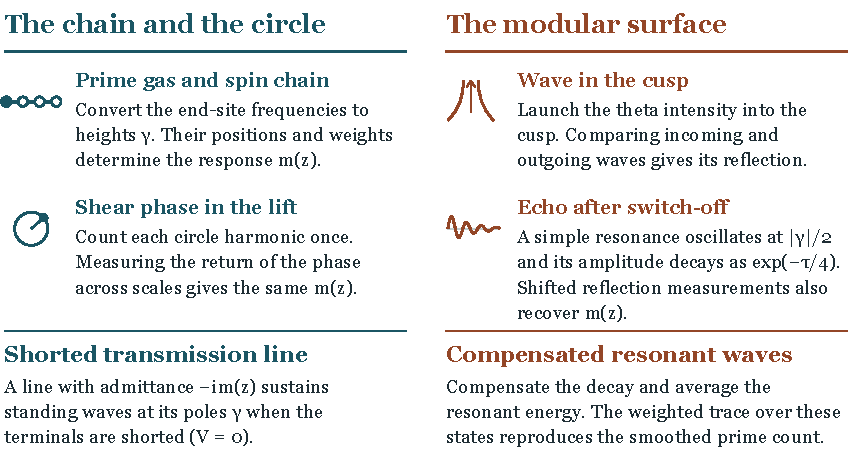
\includegraphics[width=\linewidth]{figures/manuscript/overview.pdf}
\caption{Three experiments reconstruct the same boundary response. The frequencies measured at the chain end and in the modular echo require different conversions. The modular wave escapes through a cusp. The electrical standing waves require a specified termination.}
\label{fig:overview}
\end{figure}

\section{Historical routes to a spectral proof}\label{sec:history}

Finding a system with real energies answers only half of Landau's question. One must also show that every zero appears in that system. There is a related counting problem in which we know how to do both.

For a curve over a finite field of $q$ elements, one can discover a spectrum by
counting points. The Frobenius map sends each coordinate $x$ of a point to $x^q$. A
point returns to itself after $n$ applications precisely when its coordinates
belong to the field with $q^n$ elements. For a smooth curve completed by its points
at infinity and connected over all field extensions, these counts determine the
numerator of its zeta function. The same counts can be expressed through
eigenvalues of Frobenius. Weil proved that each of the eigenvalues giving a zero
has absolute value $\sqrt q$. Counting thus identifies the whole set of zeros, and
the geometry explains why they obey a common constraint~\cite{weilcurves,deligne}.

On a compact surface of constant negative curvature, the squared frequencies of
waves traveling at unit speed are the eigenvalues of the Laplacian. Selberg showed
that a weighted sum over these levels equals an area term plus a sum over paths
that close after traveling straight on the surface (closed geodesics), including
their repetitions. The length of a geodesic on its first circuit plays the part of
$\log p$ in Riemann's formula. The exact relation depends on the surface. For the surface's own zeta function, each Laplace eigenvalue $\lambda$ gives spectral zeros satisfying $s(1-s)=\lambda$. An eigenvalue below $1/4$ therefore gives real solutions on either side of $1/2$. The surface also contributes zeros determined by its topology~\cite{selberg}.

For the Riemann zeros themselves, some of the clearest evidence for a quantum
interpretation came from their spacings. Assuming the Riemann hypothesis,
Montgomery calculated how often pairs occur at a given separation, as tested by
functions with Fourier support in $(-1,1)$. Odlyzko computed zeros high on the
critical line and found that the distribution of neighboring gaps, in units of the
mean spacing, closely followed the prediction for a family of random Hermitian
matrices called the Gaussian unitary ensemble~\cite{montgomery,odlyzko}. Berry and
Keating accounted for the leading terms in the mean number of zeros by counting
states semiclassically for $H=xp$. This motion stretches position and contracts
momentum, and the count requires cutoffs in phase space~\cite{berry}. Such averages
can agree even when individual levels differ.

An older scattering experiment gives each zero individually. Waves on the modular
surface can leave through its cusp, an open end along which a pulse can travel
arbitrarily far. Lax--Phillips scattering theory isolates the part of the wave
still interacting with the surface. In 1974 Lax and Phillips explicitly associated the critical line with decay rate $1/4$ and formulated a decay condition for a dense set of initial waves~\cite{laxphillips}. Uetake later identified the eigenvalues of the
reduced generator as $-\rho/2$, including the order of each zero~\cite{uetake}.
An open system can have many different decay rates. The correspondence therefore
identifies every zero while leaving room for one away from the critical line.
Section~\ref{sec:cusp} returns to this experiment once the prime estimate has
fixed the rate.

Weil's explicit formula gives a stronger test because it relates the primes to a
sum over all the individual zeros. Applied to the autocorrelation of a pulse (its
overlap with a shifted copy), it gives a number computed from the primes and the
completion terms. Weil's criterion in its modern form says that the Riemann
hypothesis holds exactly when this number is nonnegative for every smooth pulse of
finite duration. It can then serve as a squared
norm~\cite{weilcriterion,suzukiglobal}. Zagier found an operator with an eigenvalue
$\rho(1-\rho)$ for every zero $\rho=\beta+i\gamma$. The imaginary part of that
eigenvalue is $\gamma(1-2\beta)$. An inner product giving positive norms and
respecting the symmetries of the functions on which it acts would make the operator
symmetric, hence its eigenvalues real. Since $\gamma\ne0$, that would force
$\beta=1/2$. Finding this inner product was the open step~\cite{zagier}.

Connes obtained the zeros on the line as missing frequencies in an absorption
spectrum. In his model a hypothetical zero off the line would appear as a
resonance. He proved a version of the trace identity using finitely many primes and
identified the global identity needed to include them all~\cite{connes}. Meyer
built an operator whose spectrum contains every zero, with its order as algebraic
multiplicity. The space in which it acts allows complex
eigenvalues~\cite{meyerphysics}. De Branges proposed sufficient positivity
inequalities. Conrey and Li exhibited a failure of a proposed inequality for the
space attached to zeta~\cite{conreyli}. With the positivity in Weil's criterion as
an assumption, Suzuki constructed a self-adjoint operator by selecting a boundary
condition~\cite{suzukiglobal}. A spectral proof needs the same construction to
account for every zero and to give positive norms, with neither step assuming where
the zeros lie.

Alp\"oge's argument establishes the missing control over the primes by comparing
two estimates for the same arithmetic object. Stepanov's method for curves gains
accuracy by requiring an auxiliary function to have a zero of high order at each
point counted. Over the integers, Alp\"oge chains theta lifts to build up
divisibility by auxiliary primes. For a single nonzero integer, each distinct prime
divisor contributes its own factor to a lower bound on the absolute value. For maps
between lattices, the corresponding comparison bounds a smoothed count of prime
powers. At counting scale $X$, a chain of $r$ lifts incurs an error of about $X/r$
at its ends and a cost of order $r$ accumulated along the chain. Taking $r$ near
$\sqrt X$ balances the two. The resulting one-sided bound, up to a factor
$X^\epsilon$, holds throughout arbitrarily late intervals of scales~\cite{alpoge,primeinput,primeguide}. Why does an upper bound suffice when many oscillations can interfere? For the completed prime fluctuation there is a positive weighted average that vanishes at every shift. Its positive and negative contributions must balance. A filter that isolates one growing mode is bounded in magnitude by this same averaging kernel. A growing mode would therefore force a positive excursion even inside one of the intervals where the arithmetic bound holds. The \hyperref[app:window]{positive-kernel argument in Appendix~\ref*{app:checks}} also covers repeated zeros. This excludes $\beta>1/2$, and reflection excludes $\beta<1/2$. With the reality of the energies established, we can ask which couplings in a quantum chain the primes determine.

\section{A Hamiltonian specified by primes}\label{sec:chain}
Imagine exciting the first site of a row of coupled spins and watching the amplitude return to that site. Separating that return signal into its component oscillations (Fourier analysis) gives a frequency for each mode that the first site can excite, together with the strength of each line. We shall choose the couplings so that the frequency tells us the height of a zeta zero and the strength tells us how many zeros lie there. The couplings come from a different, much simpler system whose energies we know at the outset.

\subsection*{What the prime gas tells us}
In that system each prime $p$ labels an independent oscillator with excitation energy $\log p$. For example, two quanta in the mode for $2$ and one in the mode for $3$ have total energy $2\log 2+\log 3=\log 12$. The factorization $12=2^2\cdot3$ tells us how to recover the occupation numbers from the energy. The same correspondence works for every positive integer $n$, including the vacuum at $n=1$. At thermal equilibrium, a state of energy $L_n$ is given weight $e^{-sL_n}$, where $s$ is the inverse temperature in our energy units. The sum of these weights is the partition function. For this gas, with Hamiltonian $L$, we can calculate it in two ways. Summing over states gives a sum over integers. Summing the geometric series for each oscillator and multiplying gives a product over primes. At inverse temperature $s>1$ these agree,
\[
 \Tr e^{-sL}=\sum_{n\ge1} n^{-s}=\prod_p(1-p^{-s})^{-1}=\zeta(s).
\]
This identity is the Euler product for the Riemann zeta function. It lets us calculate the energy fluctuations of the gas directly from the primes.

Dividing each thermal weight by the partition function $Z$ gives a probability. The first derivative of $\log Z$ with respect to inverse temperature is $-\langle L\rangle$, and the second is the energy variance. Successive derivatives give the higher energy cumulants with alternating signs. For instance, differentiating the logarithm of the product above gives the mean energy as a convergent sum,
\[
 -\frac{d}{ds}\log\zeta(s)
     =\sum_p\sum_{j\ge1}(\log p)p^{-js}\qquad (s>1).
\]
The elementary factors and the gamma function in \eqref{eq:completion} have known derivatives. Adding them to the thermal derivatives gives the derivatives of $\log\xi$. We will need those at just one temperature, $s=2$.

How can fluctuations of a gas with energies $\log n$ tell us about levels at quite different energies $\gamma$? The same function $\xi$ that we compute from the gas has a product in which each factor records a zero. In the Hadamard factorization, pairing opposite zeros cancels their exponential factors, and evenness fixes the product up to $A(0)$. At a trial energy $E=i\sqrt u$ with $u>0$, the pair at $\pm\gamma$ supplies the factor $1+u/\gamma^2$. Taking a logarithm turns the product into a sum. Its first derivative in $u$ gives $1/(\gamma^2+u)$ for each pair, and higher derivatives give successive powers of this same quantity. With $L_\xi(u)=\log\xi(1/2+\sqrt u)$ the identity reads
\begin{equation}
 \begin{aligned}
 L_\xi(u)-L_\xi(0)&=\sum_{\gamma>0}m_\gamma\log(1+u/\gamma^2),\\
 S_r(u):=\frac{(-1)^{r-1}}{(r-1)!}L_\xi^{(r)}(u)
      &=\sum_{\gamma>0}\frac{m_\gamma}{(\gamma^2+u)^r},
      \qquad r\ge1 .
 \end{aligned}
 \label{eq:powers}
\end{equation}
For the calculation we use the left side of \eqref{eq:powers}. For instance, $u=9/4$ corresponds to $s=2$, and the chain rule gives $S_1(9/4)=\xi'(2)/(3\xi(2))$. The prime gas contributes $-\langle L\rangle/3$ to this number. The right side tells us what we have computed. If the positive zeta energies are the levels of $H_+$, then $S_r$ is the trace of $(H_+^2+uI)^{-r}$. Each level enters through a bounded coordinate $\lambda_\gamma=(\gamma^2+u)^{-1}$, even when $\gamma$ is arbitrarily large. Here we use the critical-line theorem to identify the candidate energy $E_\rho$ with the real height $\gamma$. This lets us interpret the right side as moments of a quantity in $(0,1/u]$.

\subsection*{How the first two averages fix the first link}
We will use $\lambda_\gamma$ as the frequency measured at the end of the chain. To specify a return amplitude we also need the probability of finding each frequency when the excitation starts at the end site. At $u=9/4$ let $S=S_1(u)$, and assign a weight to each distinct line by
\[
   \lambda_\gamma=\frac1{\gamma^2+u},\qquad
   w_\gamma=m_\gamma\lambda_\gamma/S
\]
The weights sum to one because $S$ counts each state with weight $\lambda_\gamma$. A level with two states receives twice the weight of one state at the same frequency. This choice gives us the moments of the end-site measurement before we know a single line position. Its $n$th moment is the average of the $n$th power of the measured frequency,
\begin{equation}
 \mu_n=\sum_{\gamma>0}w_\gamma\lambda_\gamma^n
       =\frac{S_{n+1}(u)}{S},\qquad \mu_0=1 .
 \label{eq:mom}
\end{equation}

To turn those numbers into couplings, write $K$ for the chain Hamiltonian and $|0\rangle$ for the excitation on the first site. A site is one possible location of the excitation. Its amplitude can stay there or hop to a neighbor. The first moment is $\langle0|K|0\rangle$, the component of $K|0\rangle$ on the initial site. The second moment is $\langle0|K^2|0\rangle=\|K|0\rangle\|^2$. Subtracting the squared first component from the total squared length leaves $\mu_2-\mu_1^2$ for the component in a new direction. Taking that direction for site $1$ gives
\begin{equation}
 K|0\rangle=a_0|0\rangle+b_0|1\rangle,\qquad
 a_0=\mu_1,\qquad b_0=\sqrt{\mu_2-\mu_1^2}.
 \label{eq:hop}
\end{equation}
Thus the mean determines the field at the end site, and the standard deviation determines the first hopping amplitude. At $s=2$ the arithmetic data give $S=0.02302207718$, $a_0=S_2/S_1=0.001586900335$ and $b_0=0.001885187523$.

The next site comes from acting with $K$ again and removing the components on the sites already constructed. At step $n$ the vectors available are $|0\rangle,K|0\rangle,\ldots,K^n|0\rangle$. We can carry out the orthogonalization on paper by representing these vectors as the polynomials $1,x,\ldots,x^n$. Their inner products are $\langle x^i,x^j\rangle=\mu_{i+j}$, and applying $K$ means multiplying by $x$. The polynomial for site $n$ has degree $n$. Multiplication raises its degree by one, so the result has zero overlap with sites beyond $n+1$. Symmetry of $K$ gives the same restriction in the opposite direction. This is how a nearest-neighbor chain emerges from the moments. The construction is the Lanczos procedure~\cite{jacobi}. The diagonal and first off-diagonal entries specify local fields and hopping amplitudes in the one-excitation sector of an XY spin chain.

Two facts ensure that this prescription works for an infinite chain. First, the squared norm assigned to a polynomial $f$ is $\sum_\gamma w_\gamma|f(\lambda_\gamma)|^2$. A polynomial of finite degree can vanish at only finitely many points unless it is identically zero, whereas the sum has positive weights at infinitely many distinct points. Every new site therefore has positive norm before normalization. Completing the polynomials in this norm gives the chain's Hilbert space. Second, the frequencies lie in a bounded interval. On $[0,1/u]$, polynomials approximate every continuous function uniformly, so two distributions with these moments agree on every continuous test and are the same distribution.

\subsection*{The zeta energies and their multiplicities}
We can now return to the end-site observation. Each line contributes $w_\gamma e^{-it\lambda_\gamma}$ to $\langle0|e^{-itK}|0\rangle$. A measured frequency $\lambda$ gives the positive zero height by the conversion $E(\lambda)=\sqrt{1/\lambda-u}$, obtained by solving for $\gamma$ in the definition of $\lambda_\gamma$. For example, the first peak near $\lambda=0.00494950$ gives a height near $14.1347$ at our chosen $u=9/4$. Reading a level through this calibration is one operation. Making a mode accumulate phase at the calibrated energy is another. The generator for the latter is
\begin{equation}
 H_{\rm cyc}=\bigl[K^{-1}-uI\bigr]^{1/2}.
 \label{eq:unbound}
\end{equation}
The operator function in \eqref{eq:unbound} keeps the eigenvectors and assigns them their new phase rates. Local hopping implements $e^{-itK}$, whereas evolution at the zeta frequencies requires $e^{-itH_{\rm cyc}}$. One feature of the conversion requires care. Arbitrarily high zeta energies correspond to frequencies accumulating at zero. The end site assigns zero probability to $\lambda=0$ and generates the whole space under powers of $K$. Any vector in the kernel of $K$ would therefore be orthogonal to the entire space. This makes the inverse well defined on a dense domain, although unbounded. Spectral calculus gives a self-adjoint $H_{\rm cyc}$ on the states of finite second energy moment. For the end site that moment diverges,
\[
 \sum_{\gamma>0}w_\gamma\gamma^2
   =\frac1S\sum_{\gamma>0}m_\gamma\frac{\gamma^2}{\gamma^2+u}=\infty .
\]
The end site still evolves unitarily under $H_{\rm cyc}$, as does every state in the Hilbert space. It is the derivative of that evolution at $t=0$ that requires the state to belong to the operator domain.

What if several states share an energy? Project the end-site excitation into that eigenspace. Every power of $K$ multiplies the projection by a scalar, so a single initial site explores only one direction there. The chain gives one direction per distinct line. Its measured weight $\langle0|P_\lambda|0\rangle=w_\gamma$, where $P_\lambda$ projects onto the line, still records how many states contributed. Dividing the weight by the single-state value $\lambda/S$ gives the integer $m_\gamma$. To form $H_+$ we assign that many orthogonal states to the energy $E(\lambda)$. Including their partners at opposite frequencies gives $H=H_+\oplus(-H_+)$, self-adjoint on states of finite second energy moment. This realizes the determinant \eqref{eq:det} with the required multiplicities. The signed frequencies are measured about the symmetry center, and the positive branch gives a lower-bounded Hamiltonian.

How much of the spectrum could a short chain recover? Each added site lets us use two more moments of the gas. The three largest chain frequencies give estimates of the three lowest positive zeta energies. As we increase the number of sites the energy estimates improve from above (Figure~\ref{fig:chain-convergence}). With sixteen sites they give $14.134725$, $21.022040$, and $25.010858$ to six decimal places. Appendix~\ref{app:checks} gives the matrix calculation and an independent check.

Using fewer sites limits how many moments enter the calculation. Each moment still contains a convergent sum over all primes. A different construction restricts the prime data themselves. On a time interval $(-a,a)$, only prime powers $p^j\le e^{2a}$ enter Suzuki's arithmetic norm. The resulting interval operator gives an upper bound on each distinct positive energy, decreasing to that energy as the interval grows (Appendix~\ref{app:checks})~\cite{suzukiconvergence}.

\begin{figure}[!htb]
\centering
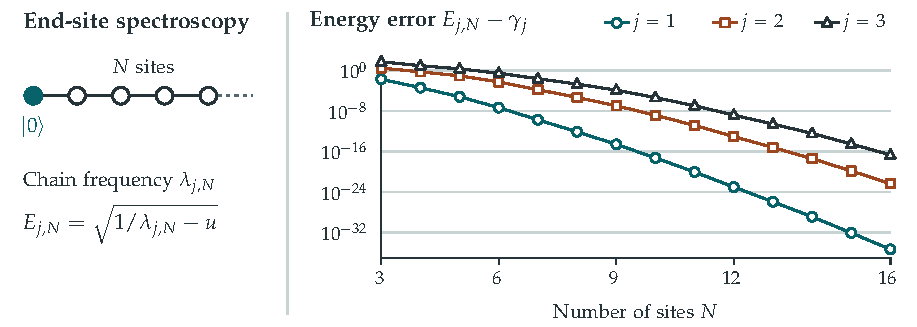
\includegraphics[width=\linewidth]{figures/manuscript/chain-convergence.pdf}
\caption{Convergence of the three lowest positive energies as the chain grows. Each measured chain frequency $\lambda_{j,N}$ gives an energy estimate $E_{j,N}$. The zero heights $\gamma_j$ enter only in the comparison on the right. The points were computed from thermal moments at 210 decimal digits and checked at 260.}
\label{fig:chain-convergence}
\end{figure}

We shall also need a way to compare this chain with other wave systems at a trial energy $z$. A suitable end-site response weights each chain mode by $[1-(z^2+u)\lambda_\gamma]^{-1}$. Its denominator vanishes when $z$ reaches either signed energy belonging to the mode. Summing these terms with their end-site weights $w_\gamma$, as in \eqref{eq:powers}, gives
\begin{equation}
 -\frac{A'(z)}{A(z)}
 =2zS\,\langle0|[I-(z^2+u)K]^{-1}|0\rangle .
 \label{eq:end}
\end{equation}
The formula packages the line positions and their strengths into one function. A line with $w_\gamma=m_\gamma\lambda_\gamma/S$ contributes $2z\,m_\gamma/(\gamma^2-z^2)$. As $z$ approaches $\gamma$, the response becomes resonant with coefficient $m_\gamma$ multiplying $1/(\gamma-z)$.

One logical step separates this construction from an independent proof of the Riemann hypothesis. To build the first link we needed a nonnegative variance, since a squared hopping amplitude cannot be negative. Building the entire chain requires a corresponding condition for every combination of the moments. If those conditions could be derived from the primes alone, the response would have poles only on the real energy axis, and every zero would have to lie on the critical line. Appendix~\ref{app:checks} states the exact inequalities and proves this implication. Here Alp\"oge's theorem gives us the required positivity. We can now ask how the signed energies behave in time.

\section{The primes in the quantum time evolution}\label{sec:primewave}
Imagine letting a system evolve for a time $t$ and keeping a reference against which to read its phase. A Ramsey experiment puts the two histories into one quantum superposition. A reference qubit prepared in $(|0\rangle+|1\rangle)/\sqrt2$ controls which evolution acts. In one branch the system waits with the identity applied, and in the other it evolves under $e^{-itH}$. For a system in a state of definite energy $\gamma$, the two branches acquire a relative phase $e^{-it\gamma}$. Measuring the qubit along $X$ gives either $+1$ or $-1$. Their average over many preparations is $\cos(t\gamma)$. We use time units of the reduced Planck constant divided by the chosen energy unit.

Which Hamiltonian sets this clock? At the end site of the local chain, the recorded phases are $e^{-it\lambda_\gamma}$ with weights $w_\gamma$. Here we want the phases of the \emph{signed} zeta energies $\pm\gamma$, so the controlled evolution must use the reconstructed $H$. To prepare a statistical mixture on its infinitely many levels, assign each energy eigenstate a probability proportional to $(1+\gamma^2)^{-1}$. These probabilities have finite sum $Q=\Tr(1+H^2)^{-1}$. The density operator is $\rho_R=(1+H^2)^{-1}/Q$, and the relative phases average to the coherence
\[
 R(t)=\Tr(\rho_R e^{-itH})
     =\frac{1}{Q}\sum_{\gamma}\frac{m_\gamma e^{-it\gamma}}{1+\gamma^2}.
\]
Each energy contributes once for each of its $m_\gamma$ states. Opposite energies have equal probabilities, so the imaginary parts cancel and the measured mean $X$ is exactly $R(t)$. The density operator itself stays stationary in each branch because it commutes with $H$. It is the changing phase between branches that produces the time signal in Figure~\ref{fig:ramsey-readout}.

Where should a prime appear in that signal? First consider what would happen if every eigenstate contributed with unit weight. Adding the phases would give the \emph{wave trace}, the Fourier transform of the density of states. Each pair of energy levels would contribute $m_\gamma(e^{-it\gamma}+e^{it\gamma})$. The infinite sum is well defined when averaged against a smooth window $\phi$ of compact support, whose Fourier transform suppresses the highest energies,
\[
 W[\phi]=\Tr\!\int \phi(t)e^{-itH}\,dt
         =\sum_\gamma m_\gamma\widehat\phi(\gamma),
 \qquad \widehat\phi(E)=\int \phi(t)e^{-itE}\,dt .
\]
The Weil explicit formula evaluates this same average using primes~\cite{connesmarcolli}. For a window supported at positive times it gives
\begin{equation}
 W(t)=e^{t/2}-\frac{e^{-5t/2}}{1-e^{-2t}}
      -\sum_p\sum_{j\ge1}\frac{\log p}{p^{j/2}}\,\delta(t-j\log p).
 \label{eq:wave}
\end{equation}
The first two terms form a smooth background $W_{\rm reg}$ due to the pole of $\zeta$ and its gamma factor. The delta function says exactly what a window centered on a prime power picks up. Its contribution is $-(\log p)p^{-j/2}\phi(j\log p)$. For example, a prime $p$ enters at $\log p$, its square at $2\log p$, and its cube at $3\log p$.

These times follow from the product over primes introduced in Section~\ref{sec:chain}. Taking its logarithm gives $\log\zeta(s)=\sum_{p,j}p^{-js}/j$ for $\operatorname{Re}s>1$. The negative derivative cancels the factor $1/j$ and supplies $\log p$ at every repetition. On the critical line $s=1/2-iE$, the factor $p^{-js}=p^{-j/2}e^{iE j\log p}$ oscillates with frequency $j\log p$ as a function of $E$. Fourier transformation puts that oscillation at the corresponding time. The explicit formula justifies this calculation after time averaging. In Selberg's trace formula a trajectory traverses the same closed geodesic several times. Here the repetitions arise in the prime product itself. Appendix~\ref{app:checks} examines which motions actually return.

The preparation determines how the ideal impulses appear at the qubit. Applying $1-\partial_t^2$ to an energy phase multiplies it by $1+\gamma^2$, exactly undoing the weighting in $\rho_R$. Thus $(1-\partial_t^2)R=W/Q$ in the sense of distributions. The coherence is continuous because its weighted phase sum converges absolutely. An impulse in its second derivative therefore shows up as a corner. The slopes immediately before and after $t_0=j\log p$ differ by
\begin{equation}
 R'(t_0^+)-R'(t_0^-)=\frac{\log p}{Q p^{j/2}} .
 \label{eq:kink}
\end{equation}
The qubit need not return to its initial reading at that instant. An exact revival would require all the occupied phases to align. The prime-power time specifies the change in their collective slope.

\begin{figure}[!htb]
\centering
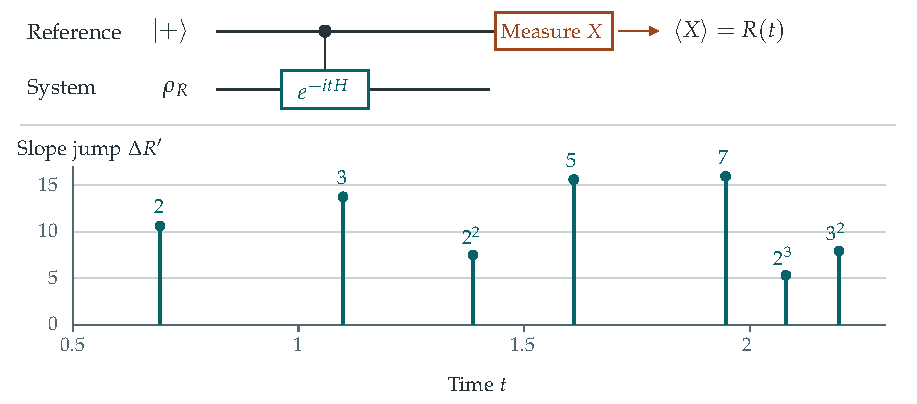
\includegraphics[width=\linewidth]{figures/manuscript/ramsey-readout.pdf}
\caption{The mean Pauli $X$ of the reference qubit gives $R(t)$ under controlled evolution of the signed system. Each stem gives the ideal jump in $R'(t)$ at $t=\log(p^j)$ from \eqref{eq:kink}. The labels identify the prime powers, including the first three powers of two.}
\label{fig:ramsey-readout}
\end{figure}

\subsection*{Resolving the first prime time}
A sum of finitely many oscillations has a continuous slope. In fact, finite mean absolute energy already guarantees this smoothness, since the differentiated sum then converges uniformly. The ideal preparation evades that condition. Its probabilities sum to one, but the growth of the number of zeros with energy gives
\[
 \Tr(\rho_R|H|)=\frac{1}{Q}\sum_\gamma\frac{m_\gamma|\gamma|}{1+\gamma^2}=\infty .
\]
For an apparatus restricted to $|\gamma|\le T$, retain those levels and renormalize their probabilities. The coherence $R_T(t)$ then rounds the corner at $t_0=\log2$ as in Figure~\ref{fig:ramsey-corner}. The omitted probability is $\epsilon_T=Q^{-1}\sum_{|\gamma|>T}m_\gamma/(1+\gamma^2)=O(\log T/T)$ by partial summation of the zero count. Both the retained and omitted phases have normalized means of magnitude at most one. Dropping the latter therefore changes the signal at any time by at most twice their probability,
\[
  \sup_t |R_T(t)-R(t)|\le 2\epsilon_T .
\]

\begin{figure}[!htb]
\centering
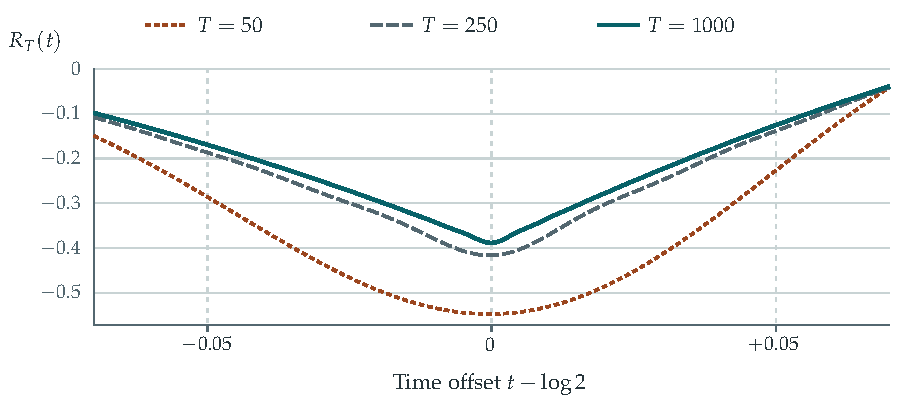
\includegraphics[width=\linewidth]{figures/manuscript/ramsey-corner.pdf}
\caption{Calculated Ramsey coherence near $t_0=\log 2$. Each curve uses the zero heights up to the stated cutoff and renormalizes the state. The three cutoffs retain 10, 108 and 649 pairs of energies, respectively. Vertical guides mark the three sampling times for $h=0.05$.}
\label{fig:ramsey-corner}
\end{figure}

Three readings suffice to compare the slopes. Measure the qubit at $\log 2-h$, $\log 2$, and $\log 2+h$. Subtract the slope through the first two readings from the slope through the last two. Smaller $h$ zooms in on the corner, but also magnifies the error in each reading. With $h=0.05$, an energy cutoff $T=25\,000$ and an absolute precision of $10^{-3}$ on each mean, the inferred jump differs from the ideal one by less than $25\%$. At each of the three times, $9.6$ million independent shots suffice to reach that precision simultaneously with at least $95\%$ confidence. These are repetitions of an ideal qubit measurement. Preparing the energy mixture and implementing the controlled evolution under $H$ are separate requirements. Appendix~\ref{app:checks} derives the error and shot bounds.

\subsection*{Predicting the qubit reading from the primes}
So far we have read prime times from a quantum signal. A second preparation reverses the calculation. Given the primes up to a specified size, we can predict what the qubit will read throughout a specified time interval. We use the same qubit and the same timing. Only the probabilities assigned to the energy levels change.

The smoothed prime count in the arithmetic proof~\cite{primeinput,primeguide} assigns each zero $\rho=\tfrac12+i\gamma$ the weight $1/[\rho(1-\rho)]=1/(\tfrac14+\gamma^2)$. Preparing the system with precisely these weights gives the density operator
\[
 \rho_*=\frac{(H^2+\tfrac14 I)^{-1}}{Z_*},\qquad
 Z_*=\Tr(H^2+\tfrac14 I)^{-1}=2+\gamma_{\rm E}-\log(4\pi),
\]
where $\gamma_{\rm E}$ is Euler's constant. The arithmetic input is a ramp beginning at $t=\log n$ for each prime power $n=p^j$. Writing $\Lambda(p^j)=\log p$ and $\Lambda(n)=0$ otherwise, the smoothed excess at time $t\ge0$ is
\[
 \mathcal E_\Lambda(t)=\sum_{n\le e^t}\Lambda(n)(e^t/n-1)-te^t+(1+\gamma_{\rm E})e^t .
\]
Each zero contributes its phase to the explicit formula for this excess with exactly the weight in $\rho_*$. Appendix~\ref{app:checks} derives the resulting prediction for the measured mean $X$, $R_*(t)=\Tr(\rho_*e^{-itH})$,
\begin{equation}
 R_*(t)=\frac{e^{-t/2}}{Z_*}
 \left[\mathcal E_\Lambda(t)-\log(2\pi)
       +\sum_{k=1}^\infty\frac{e^{-2kt}}{2k(2k+1)}\right].
 \label{eq:primecoherence}
\end{equation}
The sum over $k$ accounts for the known trivial zeros. The first term in the prime sum is easy to recognize. The factor $e^t/2-1$ is zero at $t=\log 2$ and grows smoothly thereafter. The ramp therefore starts at zero height, and its onset changes the slope. At $t=\log 2$ the predicted reading is $R_*(\log 2)=-0.3752242883\ldots$. At any later time $t$ only ramps with $n\le e^t$ have begun. Hence the prime powers through $e^{t_{\max}}$ determine the entire ideal record up to $t_{\max}$.

Equation~\eqref{eq:primecoherence} gives us more than a list of frequencies against which to test a wave system. Primes alone predict a signed answer at every time. In particular, two copies of the signal prepared a time $\log 2$ apart have a negative overlap. A system reproducing the entire record must also supply its weights, including the linear factor in the order of a repeated zero. We can now ask what a wave in the arithmetic proof can actually do.

At $t=4\log k$ the prime sum in \eqref{eq:primecoherence} is $\mathcal E_\Lambda(4\log k)=G(k^4)$ in Crossley's fourth-power criterion~\cite[Theorem~11.1]{crossleyquartic}. This criterion characterises RH by counting the integers $k$ in $[L^2,L^3]$ for which $G(k^4)>c k^{4\theta}$.

\section{The wave supplied by the theta lift}
\label{sec:lift}

In the chain we chose the couplings to reproduce the arithmetic data. The theta integral already carries a wave and a specified action on it. Two motions matter here. A shear displaces the wave along an orbit. A dilation stretches the orbit and changes the frequency of a tone along it. First we need a tone whose phase a detector can actually follow.

\subsection*{Reading a phase from the wave}

The last step of the theta lift takes an input wave $\varphi$ to an output wave $F$. For a chosen test function $\Phi$, which fixes the kernel, the integral is
\[
 F(g)=\int_{[U(W)]}\varphi(h)\,\theta_\Phi(g,h)\,dh .
\]
Here $h$ labels the input points over which we integrate, identifying points related by rational symmetries. To sample the output, start at $g_0$ and move along a \emph{shear}. The resulting signal is $F(n_u g_0)$, where successive displacements add, $n_b n_u=n_{b+u}$. Rational displacements give equivalent points, so the parameter $u$ ranges over a compact group $[N]$ with uniform probability measure $du$.

As with a periodic waveform, we can isolate a tone by multiplying by its conjugate phase $\overline{\psi(cu)}$ and averaging over $u$. Write $W_cF(g_0)$ for this complex amplitude at frequency $c$. There is a genuine tone to measure. Appendix~\ref{app:weights} shows that some output has $W_cF(g_0)\ne0$ for some $g_0$ and $c\ne0$. Shifting the waveform by $b$ and dividing by the amplitude before the shift gives~\cite{thetaoriginal}
\begin{equation}
 \frac{\int_{[N]}\overline{\psi(cu)}F(n_{u+b}g_0)\,du}
      {W_cF(g_0)}=\psi(cb)=:z(b).
 \label{eq:circle}
\end{equation}
For real displacements this ratio is $e^{i\omega b}$, with $\omega\ne0$. It serves as a phase dial. At zero displacement it reads $1$, and one turn corresponds to a displacement $2\pi/|\omega|$. Uniform measure on $[N]$ gives uniform angle on the dial. A single tone of the wave is sufficient to read the angle. The functions $z^n$ are its harmonics. As the dial makes one turn, the phase $z^n$ makes $n$ turns.

A dilation changes a shear displacement $b$ into $e^t b$. Could this scale change itself be the clock that generates the tones in \eqref{eq:primecoherence}? Suppose a single step multiplies every nonzero shear frequency by a prime $p$. It shifts the band $1\le |q|<p$ to the next band, and likewise for every band $p^j\le |q|<p^{j+1}$. A standing mode would have to carry equal power in all of them. Their sum could be finite only if that power were zero. At the marked real place the finite-norm sector has no constant shear mode left over. Appendix~\ref{app:resonance} proves this fact and the decay of any fixed linear pickup under the original dilation. Over a prescribed finite interval a suitable packet can still reproduce the recurrent signal (Appendix~\ref{app:checks}).

The lift supplies more than this one motion. The shear acts on a rational plane inside the data of the integral. Its rational symmetries let us use the lift to prepare a pulse on the modular surface. The pulse then propagates according to that surface's wave equation. We return to the phase circle in Section~\ref{sec:line}.

The lift itself conserves a source-to-detector amplitude. Given an input and a detector at the final output, we can propagate the input through some of the integrals and the detector backwards through the rest. Their complex overlap gives the same reading wherever they meet, because the reverse maps are the adjoints of the forward maps. Summing over a full basis of detectors gives a conserved squared norm for the output visible at the end. Moving the meeting point leaves that output exactly as it was. To observe a wave losing energy in time we need an evolution. The marked plane of the lift supplies a source for the following one.

\section{What decays on the modular surface}\label{sec:cusp}

An echo gives two pieces of information. The interval between peaks tells us how fast a wave oscillates. The envelope of those peaks tells us how fast the oscillation dies away. On the modular surface these are the two coordinates of a zeta zero. To see where the arithmetic enters, consider the surface in Figure~\ref{fig:modular-wave}. Points related by integer matrices of determinant one represent the same point. Gluing the indicated sides together leaves one end through which a wave can escape, the \emph{cusp}. Far up the cusp its horizontal coordinate is periodic. If we average over one period, the wave equation on the surface reduces to the ordinary one-dimensional wave equation along the cusp. More precisely, with nonnegative hyperbolic Laplacian $\Delta$, the equation is $u_{\tau\tau}=(-\Delta+1/4)u$. The traveling wave is the horizontal average divided by $\sqrt y$, and its distance coordinate is $\log y$. We can therefore send a wave in and compare what comes back.

\begin{figure}[!htb]
\centering
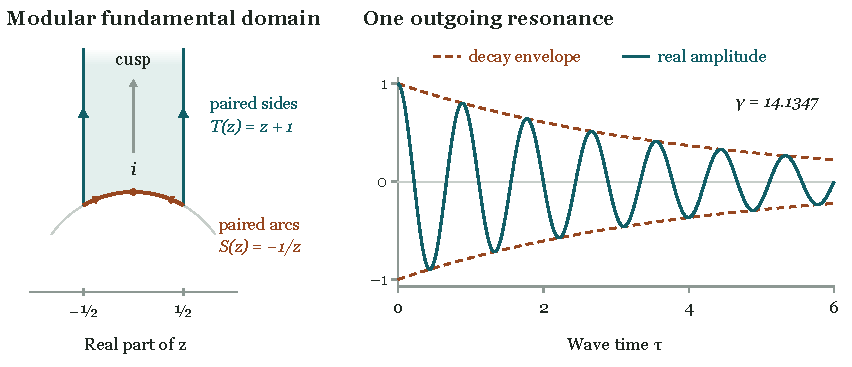
\includegraphics[width=\linewidth]{figures/manuscript/modular-wave.pdf}
\caption{Left: identifying the indicated sides of the hyperbolic plane domain produces the modular surface. The cusp extends to infinite height. Right: the real amplitude of one outgoing resonance, $e^{-\tau/4}\cos(\gamma\tau/2)$, at the lowest positive zeta height. A pulse containing many modes generally has a more complicated envelope.}
\label{fig:modular-wave}
\end{figure}

An incident height profile $y^s$ must respect the identifications of the surface. Adding all its distinct images gives a field called an \emph{Eisenstein series}. A matrix that makes an image has a bottom row $(c,d)$ of relatively prime integers. For $c>0$, the number of possible residues $d$ modulo $c$ is Euler's totient $\varphi(c)$. Each residue contributes the same integral to the horizontal average. The result has an incident and a reflected term, $y^s+\phi(s)y^{1-s}$, with
\begin{equation}
 \phi(s)=\frac{\sqrt\pi\,\Gamma(s-\tfrac12)}{\Gamma(s)}
             \sum_{c\ge1}\frac{\varphi(c)}{c^{2s}}
       =\frac{\sqrt\pi\,\Gamma(s-\tfrac12)}{\Gamma(s)}
             \frac{\zeta(2s-1)}{\zeta(2s)} .
 \label{eq:cusp-reflection}
\end{equation}
The series converges for $\operatorname{Re}s>1$. Its Euler product gives the second equality. With time convention $e^{-i\omega\tau}$, put $s=1/2-i\omega$. The normalized profiles are then the incoming $e^{-i\omega\log y}$ and outgoing $e^{i\omega\log y}$ waves~\cite{muellerspec}. The zeta function thus enters the reflected wave through a count of the integer rows permitted by the geometry.

The marked plane in the theta integral gives us a way to launch the pulse. Its two null directions support a rational action of $\mathrm{SL}_2$, the group of determinant-one matrices. Restrict a nonzero output wave to this group near a point where the wave is nonzero. Its intensity is positive there. Averaging the intensity over rotations and over the finitely many sheets of its arithmetic cover gives a nonzero intensity on the modular surface. Use a smooth observation window around the point to make the source $f$ of finite extent. We use the component of $f$ in the continuous spectrum as the initial velocity, removing the spatially constant mode as well as discrete standing waves. Why can one pulse reveal a property of the surface? Its overlap $P_f(s)$ with the Eisenstein wave satisfies $P_f(s)=\phi(s)P_f(1-s)$. For real $s>1$ the overlap is positive, since both the intensity and the Eisenstein wave are nonnegative and the source is nonzero. Analytic continuation then makes it nonzero at almost every real scattering frequency. The source cancels in the ratio of the complete records, even if its particular echo misses an isolated resonance. Appendix~\ref{app:resonance} gives the construction. We use the phase convention of the two height profiles in \eqref{eq:cusp-reflection}.

To measure a lifetime, follow the part of the signal still interacting with the surface. Uetake removed the freely traveling components and one known elementary mode. He proved that the resulting generator $A_c$ has eigenvalues $-\rho/2$, each with algebraic multiplicity equal to the order of $\rho$~\cite[Theorem~4.4]{uetake}. For $\rho=\beta+i\gamma$ an eigenmode therefore evolves in wave time $\tau$ as
\begin{equation}
                 e^{-\beta\tau/2}\,e^{-i\gamma\tau/2}.
 \label{eq:cusp-decay}
\end{equation}
Wave energy can escape at many rates on an open surface. Alp\"oge's prime bound fixes $\beta=1/2$ for every mode. Thus however high the tone, its amplitude has the same exponential decay rate $1/4$. Generalized modes at a repeated zero can also have a polynomial prefactor. The self-adjoint Laplacian's square-integrable standing waves belong to a different part of the spectrum.

What fixes the value $1/4$? For an algebraic period measured by the lift, the product formula equates its total logarithmic size at the complex embeddings to its total divisibility at the finite primes (Appendix~\ref{app:cut-period}). This exact balance lets the size estimates bound a prime count. To see the importance of their precision, suppose the resulting error at scale $X$, with $r$ lifts, were $X/r+r^2$ up to $X^\epsilon$. Optimizing $r$ would give exponent $2/3$, provided the other errors respected that bound~\cite[\S I.8]{primeguide}. The positive filter of Appendix~\ref{app:window} would then give $\beta\le2/3$, and reflection would give $\beta\ge1/3$. A whole band of decay rates, from $1/6$ to $1/3$, would be allowed by this estimate. The sharper arithmetic estimate has cost $X/r+r$. Its exponent is $1/2$, where the two ends of the band meet at $1/4$. It is this gain in the arithmetic estimate that selects the rate.

A pulse made of many resonances can behave quite differently from a single tone. Two modes with opposite amplitudes at the exit lose no energy at that instant. There are enough closely spaced tones to sustain destructive interference. For any prescribed finite duration one can prepare a pulse in the resonance space that retains as near to all its initial squared norm as desired. Appendix~\ref{app:outgoing-flux} derives this directly from the outgoing wave equation. For a concrete example, the $222$nd, $223$rd and $224$th positive resonances each retain $13.53\%$ of their initial squared norm after four units of wave time. In the superposition specified in the appendix the retained fraction is $85.75\%$. Figure~\ref{fig:cusp-retention} shows the two readings. The three-tone preparation uses the indicated frequencies and phases.

\begin{figure}[!htb]
\centering
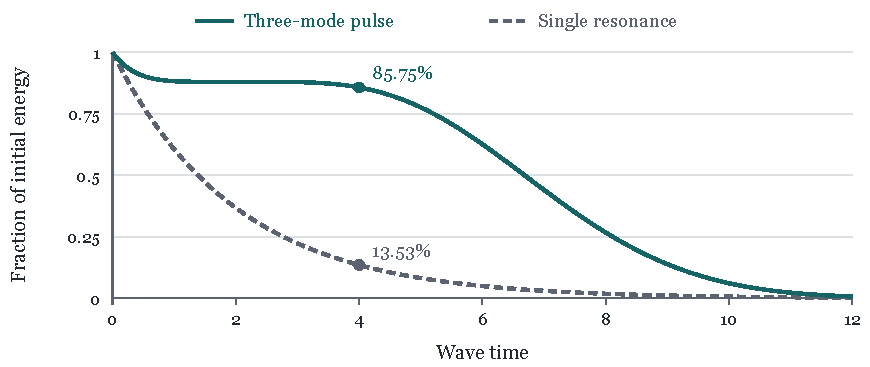
\includegraphics[width=0.92\linewidth]{figures/manuscript/cusp-retention.pdf}
\caption{Remaining squared norm in the outgoing scattering space. Every individual resonance follows the dashed curve. For the solid curve, three resonances are phased so that both their combined exit amplitude and its first derivative vanish at wave time two. The loss is small while they cancel at the opening.}
\label{fig:cusp-retention}
\end{figure}

\subsection*{Recovering the spin-chain response from one cusp}
Does the cusp tell us the strengths measured by the spin chain? Remove the elementary geometric factor in \eqref{eq:cusp-reflection} and denote the reduced reflection by $C$. Write $g=\xi'/\xi$. In the convention of that equation,
\begin{equation}
 C(q)=\frac{q-1/2}{q+1/2}\,\phi(1/2+q)
     =\frac{\xi(2q)}{\xi(1+2q)},\qquad
 \frac12\frac{C'(w/2)}{C(w/2)}=g(w)-g(w+1).
 \label{eq:cusp-shift}
\end{equation}
These meromorphic identities follow from the completion in \eqref{eq:completion}. The last one has a useful measurement interpretation. At $w=1/2-iz$ a slope of the reflection gives the difference between $g$ at two damping settings. Add the differences at $w,w+1,\ldots,w+N-1$. The intermediate terms cancel. In $g(w+N)$ the elementary and gamma factors are known and $\zeta'/\zeta(w+N)$ tends to zero. This recovers the chain response $m(z)=i\,g(w)$ without fitting individual resonances. At $z=10+i,20+i,30+i$, summing 32 differences reproduced the independently integrated phase-circle response of Section~\ref{sec:line} to within $5.71\times10^{-11}$ in each case. Appendix~\ref{app:resonance} gives the truncation bound. Finite, noisy records introduce a separate measurement error.

\subsection*{What survives the loss}
The prime count predicts an oscillation that persists, while an individual modular echo decays. To compare the two, compensate the measured amplitude by $e^{\tau/4}$ and measure time in units $t=\tau/2$. Distinct modes now carry phases $e^{-i\gamma t}$. Their wave profiles need not be orthogonal, so the squared norm of their sum still contains beats. Taking its long-time average removes the cross terms. Appendix~\ref{app:resonance} shows how to retain the successive powers of time at repeated resonances. The resulting conservative evolution has a self-adjoint generator $H_{\rm mod}$, with one state for every zero counted with its order.

The prime count also tells us how strongly to weight these states. Each occurrence of a zero contributes $1/[\rho(1-\rho)]$ to the smoothed count in \eqref{eq:primecoherence}. For one state at a critical-line zero this weight is exactly the squared modulus of $(1/2+i\gamma)^{-1}$. Weight the compensated modes accordingly and average their phases. With $D_*=(\tfrac12+iH_{\rm mod})^{-1}$ the result is
\begin{equation}
       R_*(t)=\frac{\Tr(D_*^*D_*\,e^{-itH_{\rm mod}})}{\Tr(D_*^*D_*)}.
       \label{eq:cusp-prime}
\end{equation}
The left side can be calculated using just the prime powers through $e^{|t|}$. On the right the frequencies and their multiplicities come from modular scattering. This agrees at every time, including the sign of the interference. It is a collective measurement of compensated resonances. An ordinary pulse left on the surface continues to radiate.

\section{From the phase circle to a transmission line}\label{sec:line}

The cusp gave us $m$ through a ratio of waves traveling in opposite directions. The phase dial of Section~\ref{sec:lift} offers a second route to the same function, and this one makes contact with a laboratory boundary condition. We first have to decide what a return to the initial phase will measure.

\subsection*{Counting and measuring the shear harmonics}

Consider a return experiment on this circle. Start each trial at phase $1$, apply a random real displacement $b$, and read the phase again. Choose $b$ Gaussian with mean zero and variance $2t/|\omega|^2$. Here $t$ sets the strength of the imposed phase diffusion. The unwrapped angle $\omega b$ has variance $2t$, so its $n$th Fourier moment is $\mathbb E[e^{in\omega b}]=e^{-tn^2}$. How often does the dial return near its starting point? Count the trials ending in a small arc around $1$ and divide the resulting fraction by the fraction of the circle occupied by the arc. As the arc shrinks, the ratio approaches the return density relative to uniform angle. Fourier inversion at the starting point gives $1+2\sum_{n\ge1}e^{-tn^2}$. Each harmonic enters with unit weight because preparation and detection use the same phase point, so their Fourier factors multiply to $z^n\overline{z^n}=1$. The factor two counts the two signs and the constant harmonic supplies the one.

Set $t=\pi r^2$, where $r>0$ controls the spread of the random displacement. On the positive harmonics let $N z^n=n z^n$, so $N^2$ is the kinetic energy in units set by the fundamental frequency. Removing the constant and combining the two signs gives the heat trace
\begin{equation}
 h(r)=\Tr e^{-\pi r^2N^2}=\sum_{n=1}^\infty e^{-\pi n^2r^2}.
 \label{eq:heatcount}
\end{equation}
Varying $r$ changes the probe of this fixed spectrum. A general rescaling of $N$ would change its eigenvalues and could not be a unitary conjugation. The same count respects every prime covering of the circle. The map $z\mapsto z^p$ takes the orthonormal modes $z^n$ isometrically to $z^{pn}$. Any count preserved by these maps satisfies $a_{pn}=a_n$ for every prime $p$ and hence, by factorization, $a_n=a_1$. The return experiment gives $a_1=1$.

The return density can also be calculated by adding the ordinary Gaussian densities at all displacements that give a whole number of turns. Equating the result to its Fourier series is Poisson summation. With our choice of $t$ the Gaussian is its own Fourier transform at unit scale, and the resulting reciprocal-scale identity is
\[
 1+2h(r)=r^{-1}\,[1+2h(1/r)] .
\]
For small $r$, modes with $n$ up to order $1/r$ contribute, and $h(r)\sim1/(2r)$.

What if we listen directly for those harmonics in the original wave? Keep one observation point $g_0$ and one set of wave symmetries and boundary data throughout the measurement. Appendix~\ref{app:weights} makes precise this choice of a fixed automorphic level and type. These choices leave finitely many independent input copies. Excite an orthonormal basis of inputs and sum the powers of their output waves $F_j$ at each frequency $nc$. The result $w_n=\sum_j|W_{nc}F_j(g_0)|^2$ is independent of the basis. This measures the total intensity of the $n$th tone over the independent inputs. Appendix~\ref{app:weights} gives the equivalent formula using the lift and its adjoint~\cite{stagebasis}. Parseval's identity bounds the total power in these harmonics by the power of the waves on the entire orbit,
\begin{equation}
 0<M:=\sum_{n\ge1}w_n\ \le\
 \sum_j\int_{[N]}|F_j(n_b g_0)|^2\,db<\infty .
 \label{eq:power}
\end{equation}
The tone used to set the dial gives $w_1>0$. Equal power at every multiple of that frequency would make the sum infinite. This difference from the return measurement shows up directly in a scan over $r$. With constant-mode weight $w_0\ge0$, let $\vartheta_w(r)=w_0+2\sum_{n\ge1}w_ne^{-\pi n^2r^2}$. Smoothness gives $\sum n^2w_n<\infty$. As $r$ decreases, the measured power approaches $w_0+2M$ with error $O(r^2)$. At reciprocal scale $1/r$ only the constant mode survives to this accuracy. Hence
\begin{equation}
 \vartheta_w(r)-r^{-1}\vartheta_w(1/r)
    =-w_0/r+w_0+2M+O(r^2).
 \label{eq:defect}
\end{equation}
Even setting $w_0=0$ leaves a discrepancy of $2M$ in the limit.

A larger collection of theta waves might fill in the missing power. The available estimates control how it is shared on average. A detector could still miss an individual harmonic completely, as the calculation in Appendix~\ref{app:weights} shows.

There is a second way to read each term of $h(r)$ from the lift. Follow the same tone as a dilation changes its frequency. The rational dilation $d(a)$ multiplies a shear displacement by $a^2$. Rational invariance then makes the coefficient at frequency $n^2c$ and point $d(1/n)g_0$ equal to the original $W_cF(g_0)$. At that setting the phase advances as $e^{in^2\omega b}$. Averaging over $b$ with a Poisson kernel of width $\pi r^2/|\omega|$ gives $e^{-\pi n^2r^2}$ (Appendix~\ref{app:weights}). In Figure~\ref{fig:moving-detector} each row is a different setting. Giving each row one count reproduces the return density's positive-harmonic sum.
\begin{figure}[!htb]
\centering
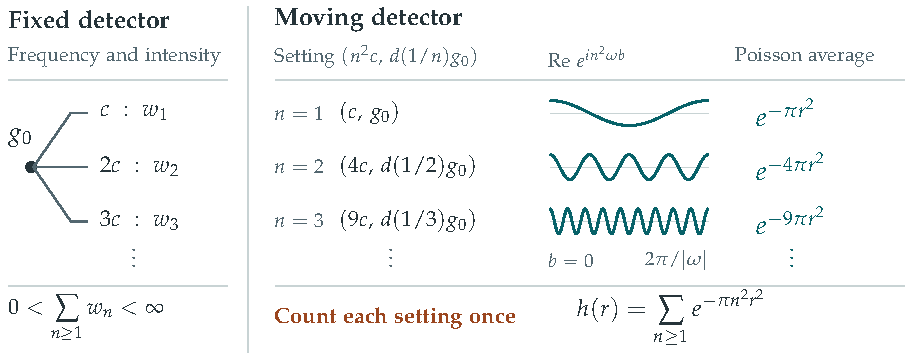
\includegraphics[width=\linewidth]{figures/manuscript/moving-detector.pdf}
\caption{The fixed detector measures harmonic power in the wave at one point. Moving the detector follows a single coefficient. At the first three settings its initial amplitude is the same, but its phase runs through $1$, $4$ and $9$ cycles per fundamental shear period. Poisson averaging gives one Gaussian factor in each row.}
\label{fig:moving-detector}
\end{figure}

\subsection*{From the heat trace to the boundary response}

We now have a record $h(r)$ of returns as a function of scale. To find its frequency content under changes of scale, use $x=\log r$, so doubling $r$, for example, adds $\log 2$ to $x$. Integrating the record against $r^s\,dr/r$ gives its Mellin transform. For harmonic $n$, the change of variable from $r$ to $nr$ leaves the same Gaussian integral times $n^{-s}$. Summing these factors gives $\tfrac12\pi^{-s/2}\Gamma(s/2)\zeta(s)$ for $\operatorname{Re}s>1$. At $s=\tfrac12-iE$ the integral would be the ordinary Fourier transform of $g(x)=e^{x/2}h(e^x)$. It fails to converge because $g(x)\sim e^{-x/2}/2$ as $x\to-\infty$.

Reciprocity supplies a way to remove this growing background. In logarithmic scale it gives
\[
 g(x)-g(-x)=\tfrac12(e^{-x/2}-e^{x/2}).
\]
Each background exponential has a second derivative equal to one quarter of itself. The combination $g\,\mapsto\,g''-g/4$ removes both exponentials. What remains is an even pulse. At large positive $x$ the Gaussian sum and its derivatives decay rapidly, and evenness gives the same decay at the other end. Two integrations by parts in the convergent half-plane show that this operation multiplies the Mellin transform by $(s-1/2)^2-1/4=s(s-1)$, precisely the remaining factor in \eqref{eq:completion}. The Fourier transform of the resulting pulse is consequently the same completed amplitude $A(E)$ obtained from the prime gas,
\begin{equation}
 k(x)=(\partial_x^2-\tfrac14)\,[e^{x/2}h(e^x)],\qquad
 \widehat k(E)=A(E),\qquad \mathcal F[-ix k(x)](E)=A'(E).
 \label{eq:pulse}
\end{equation}
The last equality prescribes a second reading of the same record. Before Fourier analysis, multiply each sample by its logarithmic scale $x$ and by $-i$. This measures the first logarithmic moment, since differentiating the Fourier phase $e^{-iEx}$ brings down $-ix$. The negative ratio of the second transform to the first gives the end response $m=-A'/A$ of \eqref{eq:end}.

There is a physical translation in $x$ inside the lift. A continuous dilation stretches shear displacements by $e^t$ and preserves the sign of their Fourier frequency $q$. On an occupied ray of frequencies of one sign, dilation translates $x=-\log(|q|/|\omega|)$. The affine-group representation identifies this space with $L^2(\mathbb R,dx;\mathcal M)$, where $\mathcal M$ labels independent copies. Selecting a unit vector in $\mathcal M$ picks out one scalar wave~\cite{affine}. Its frequency components can be filtered under the original integral. A real shear by $b$ gives the phase $e^{ibq}$. Averaging over $b$ with the inverse Fourier transform of a desired filter therefore applies that filter at $q$, including $k(x)$ and $xk(x)$. Absolute summability of the theta terms and decay of the input justify exchanging the integrals~\cite{thetamixed}.

The free translation has continuous spectrum, as we saw in Section~\ref{sec:lift}. Extracting $m$ from a pulse does not stop that pulse from escaping. A transmission line provides an explicit way to turn its response into a standing-wave measurement by connecting a load across two terminals.

\subsection*{Driving a transmission line}

Consider a pair of terminals at the left end, $\ell=0$, of a lossless transmission line extending to the right. Apply a voltage $V$ across the terminals and measure the current $I$ flowing into the line. We want the ratio $I/V$ at complex frequency $z$ to equal $-im(z)$. The natural frequencies of this line depend on what is connected across its terminals. An ideal voltage source set to zero and left connected holds the terminals at the same potential. This is a short circuit, $V=0$, and current can still flow through it. Disconnecting the source leaves an open circuit, $I=0$, and a voltage can develop. The wall is the condition imposed at $\ell=0$.

A passive line can store energy and return it to a source. If the line has no internal power source, its current-to-voltage ratio (the admittance) must have nonnegative real part for $\operatorname{Im}z>0$. The expansion in \eqref{eq:end} gives precisely that sign. Each positive zeta frequency $\gamma$ contributes $m_\gamma[(\gamma-z)^{-1}+(-\gamma-z)^{-1}]$ to $m(z)$, and both terms have positive imaginary part. An independently specified passive line with this exact response would exclude off-line zeros, since its admittance is analytic throughout the upper half-plane. Here we use the critical-line theorem to establish the sign and hence construct the line. The line oscillates at signed frequencies in the $\gamma$ coordinate. The hopping frequencies of the chain in Section~\ref{sec:chain} are $\lambda=(\gamma^2+u)^{-1}$.

The inverse theorem for canonical systems gives the line's equation of motion. Write the fields as $Y_1=V$ and $Y_2=iI$. The theorem supplies a real symmetric matrix $G(\ell)\ge0$ that sets the energy stored per unit length. Normalizing $\Tr G=1$ fixes the distance coordinate $\ell$ and makes $G$ unique almost everywhere~\cite{canonicalphysics}. Whereas $x$ measured the logarithmic scale of the pulse, $\ell$ measures distance from the terminals. The wave obeys
\begin{equation}
 iG(\ell)\,\partial_tY=J\partial_\ell Y,\qquad
 J=\begin{pmatrix}0&-1\\1&0\end{pmatrix}.
 \label{eq:localwave}
\end{equation}
The equation and its adjoint give the local energy balance,
\[
 \partial_t(Y^\dagger GY)+\partial_\ell j=0,\qquad j=iY^\dagger JY.
\]
The first term tracks the energy density and the second its flow. To separate a wave sent into the line from the one returning to the terminals, we resolve the endpoint flux into two contributions. At unit reference impedance the amplitudes are
\begin{equation}
 a=\frac{Y_1-iY_2}{\sqrt2},\qquad b=\frac{Y_1+iY_2}{\sqrt2},
 \qquad j=|a|^2-|b|^2 .
 \label{eq:portflux}
\end{equation}
At the terminals $a=(V+I)/\sqrt2$ is the incident amplitude and $b=(V-I)/\sqrt2$ is the reflected amplitude, both measured relative to unit impedance. Positive $j$ therefore means that the line receives more power than it returns.

What amplitude comes back? For time dependence $e^{-izt}$ the wave equation becomes $JY'=zGY$. For $\operatorname{Im}z>0$ the condition that the field have finite norm $\int_0^\infty Y^\dagger GY\,d\ell$ singles out a boundary direction. The inverse theorem gives that direction as $(1,m(z))^{\mathrm T}$, the response to unit terminal voltage. The net flux into the line is then $2\operatorname{Im}m(z)$, which gives the sign condition its physical meaning. The returning amplitude follows from \eqref{eq:portflux},
\begin{equation}
 \frac{b}{a}=\Theta(z)=\frac{1+i m(z)}{1-i m(z)}
             =\frac{A(z)-iA'(z)}{A(z)+iA'(z)} .
 \label{eq:theta}
\end{equation}
Its modulus is at most one in the upper half-plane and equals one at real frequencies, with common factors canceled at multiple zeros.

Equation~\eqref{eq:theta} describes the reflection by the medium. A wall imposes a second condition on the same endpoint amplitudes. For a lossless wall of fixed phase, write $b=\alpha a$, $|\alpha|=1$. A standing wave can persist without a drive when the two conditions agree, $\Theta(E)=\alpha$. A short gives $b=-a$, so the two voltages cancel and the standing-wave frequencies are the poles of $I/V$. An open circuit gives $b=a$, so the currents cancel and the frequencies are the zeros of $I/V$, where $A'(E)=0$ and $A(E)\ne0$. Both terminations conserve energy and preserve the pairing of signed frequencies since $\Theta(-E)=\overline{\Theta(E)}$ on the real axis.

\subsection*{Choosing the termination from a static measurement}

With an ideal voltage drive, the short is the condition left when the drive is set to zero. To ask how much of that choice follows from the lift, we can compare the line with the response of a freely dilating wave to a steady drive. Before a wall is imposed, dilation has a continuous range of frequencies. Its generator acts on a packet by $Df(E)=Ef(E)$ in $L^2(\mathbb R,dE)$. We first specify which part of each packet we want the measurement to retain. We keep the amplitudes in a single channel picked out by the measured reflection phase. The operation of keeping that part is the projection $P_\Theta$. Appendix~\ref{app:boundary} specifies the channel and computes the projected response~\cite{suzukiglobal}. This choice uses the reflection already obtained by counting the shear harmonics.

A zero-frequency drive with damping $\eta>0$ produces the free response $1/(E-i\eta)=(E+i\eta)/(E^2+\eta^2)$ at energy $E$. Its real part measures dispersion, while its imaginary part concentrates around zero as $\eta$ decreases. This narrowing peak retains area $\pi$. For a packet in the chosen channel the absorptive response approaches
\[
 \int_{\mathbb R}\frac{\eta\,|f(E)|^2}{E^2+\eta^2}\,dE
     \longrightarrow \pi|f(0)|^2 .
\]
The entire residual absorption depends on a single amplitude $f(0)$. It therefore has rank one in this channel. A self-adjoint Hamiltonian with an inverse has real static response. Our matching rule identifies that inverse with the dispersive part measured in the free dilation,
\begin{equation}
 H_{\rm s}^{-1}=C=\lim_{\eta\downarrow0}
       P_\Theta\frac{D}{D^2+\eta^2}\bigg|_{\operatorname{ran}P_\Theta}.
 \label{eq:static}
\end{equation}
Appendix~\ref{app:boundary} compares \eqref{eq:static} with the wall Hamiltonians. In operator norm the full projected resolvent approaches the inverse for the short plus the imaginary rank-one term above. Taking its self-adjoint part therefore selects $V(0)=0$. The result depends on the chosen channel and static matching rule. The cusp measurement in Section~\ref{sec:cusp} recovers $m$ before making either electrical choice.

At a signed zero $\gamma$ of order $d$, $m(E)=d/(\gamma-E)+O(1)$. The endpoint direction tends to $(0,1)^{\mathrm T}$, a nonzero current at zero voltage. Conversely, the short-circuit condition $\Theta(E)=-1$ requires a pole of $m$. This gives one standing wave at each distinct signed zero. A repeated zero still gives one wave in this scalar channel, but the slope of its reflection phase gives the order through $|\Theta'(\gamma)|=2/d$. Appendix~\ref{app:boundary} uses that integer to place $d$ orthogonal copies of the wave in the dilation space. With these copies the wall and the signed Hamiltonian reconstructed from the chain have matching energies and degeneracies. Identifying the corresponding experiments would also require matching their preparations and observables.

The closed response can be probed while the terminals remain accessible. Measure reflection phase and retain the part of a packet with $|1+\Theta(E)|<\epsilon$, $0<\epsilon<2$. For every unit packet in the selected channel the phase is uniformly distributed, so the accepted fraction equals the angular fraction $p_\epsilon=2\arcsin(\epsilon/2)/\pi$ (Figure~\ref{fig:phase-window}, Appendix~\ref{app:boundary}). Dividing by $\sqrt{p_\epsilon}$ preserves inner products because the fraction is the same for all packets. At $z=i$ the conditional resolvent approaches $(H_{\rm s}-i)^{-1}$ with error $O(\epsilon^2)$ in operator norm. Averaging symmetrically about $-1$ cancels the first-order change with phase. The cost is $1/p_\epsilon\sim\pi/\epsilon$ independent preparations per accepted packet on average.

\subsection*{Capacitance and inductance near the terminals}

The measured response tells us how the material stores energy. Its frequency symmetry fixes the principal axes of the density throughout the line, and its high-frequency behavior gives the average capacitance and inductance close to $\ell=0$. In the coordinates of \eqref{eq:portflux}, these two statements read
\begin{equation}
 G(\ell)=\begin{pmatrix}\mathcal C(\ell)&0\\0&1-\mathcal C(\ell)\end{pmatrix}
 \ \text{a.e.},\qquad
 \lim_{h\downarrow0}\frac1h\int_0^h G(\ell)\,d\ell
     =\begin{pmatrix}1&0\\0&0\end{pmatrix}.
 \label{eq:medium}
\end{equation}
The zero off-diagonal entries mean that the capacitive and inductive contributions to stored energy can be separated at every depth, up to a set of measure zero. The reason is the symmetry between positive and negative frequency. Appendix~\ref{app:boundary} shows how this symmetry fixes those axes.

In voltage and current variables, \eqref{eq:localwave} now reads
\begin{equation}
 \partial_\ell V=-\mathcal L(\ell)\,\partial_t I,\qquad
 \partial_\ell I=-\mathcal C(\ell)\,\partial_t V,\qquad
 \mathcal L=1-\mathcal C .
 \label{eq:line}
\end{equation}
These are the lossless transmission-line equations, with capacitance $\mathcal C$ and inductance $\mathcal L$ per unit length in normalized units. The stored density is $\mathcal C|V|^2+\mathcal L|I|^2$, and the flux is $2\operatorname{Re}(\bar V I)$.

The endpoint average in \eqref{eq:medium} comes from the response at high complex frequencies (Appendix~\ref{app:boundary}). In closed angular sectors inside the upper half-plane, the gamma factor of the completed zeta function produces logarithmic growth while the prime contribution becomes exponentially small. This fixes the average capacitance at one and the average inductance at zero in the limit of a shrinking interval. An entire initial layer of zero inductance would force $\operatorname{Im}m(iy)$ to grow at least linearly in $y$. Every initial interval therefore contains some inductance. On the real axis the individual resonances persist. An explicit spatial profile for the coefficients in \eqref{eq:line} and an interpretation of $\ell$ in the theta space remain open.

\subsection*{A finite circuit for a frequency band}

Ordinary resonators can reproduce a terminal measurement on a finite frequency band. The $N$-site chain of Section~\ref{sec:chain} gives a rational approximation $m_N$ in \eqref{eq:end}. A chain frequency $\lambda_j$ sets a resonance frequency $\omega_j$ in the line's units, while the probability $\nu_j$ of detecting that state at the end site sets its strength. With Laplace frequency $\sigma=-iz$ and zeta argument $s=1/2+\sigma$, the predicted admittance is
\begin{equation}
 Y_N(\sigma)=-i m_N(i\sigma)=\sum_{j=1}^N\frac{d_j\sigma}{\sigma^2+\omega_j^2},
 \qquad \omega_j^2=1/\lambda_j-u,\qquad d_j=2S\nu_j/\lambda_j .
 \label{eq:branches}
\end{equation}
Each term describes a series branch with inductance $L_j=1/d_j$ and capacitance $C_j=d_j/\omega_j^2$, both positive. If $Q_j$ is the capacitor charge, the applied voltage drives $L_j\ddot Q_j+Q_j/C_j=V$. Connecting the branches in parallel puts the same voltage across each and adds their currents $\dot Q_j$. Setting the driving voltage to zero while leaving the source connected lets every branch oscillate freely at $\omega_j$. During a driven measurement, the voltage reflection at unit reference impedance is $(1-Y_N)/(1+Y_N)$.

Figure~\ref{fig:resonators} tests the circuit over $10\le E\le30$, a band containing the first three positive zeta frequencies. Evaluating the reflection at $z=E+i$ weights the impulse response by $e^{-t}$ before Fourier analysis. For an absolute tolerance of $10^{-3}$ on the complex reflection amplitude, eleven branches suffice throughout the band. The uniform error is below $2.26\times10^{-4}$, while each of the first ten chain truncations exceeds the tolerance at the upper band edge. Appendix~\ref{app:circuit} gives the component values and includes their rounding in the bound.

\begin{figure}[!htb]
\centering
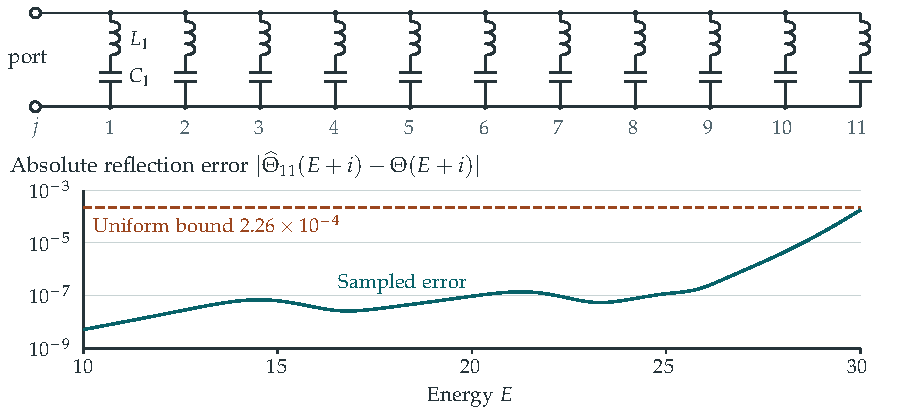
\includegraphics[width=\linewidth]{figures/manuscript/resonators.pdf}
\caption{Eleven series LC branches in parallel at the port. The solid curve joins 2,001 values of the reflection-amplitude error at $z=E+i$, computed with the rounded parameters in Table~\ref{tab:resonators}. The dashed bound includes the interpolation allowance between samples.}
\label{fig:resonators}
\end{figure}

\section{What the construction explains}
The first positive zeta height illustrates what the different instruments measure. At the end of the local spin chain the largest frequency is near $0.00494950$. With $u=9/4$, converting that measured frequency $\lambda$ gives $\sqrt{1/\lambda-u}\simeq14.1347$. The line strength gives its multiplicity. On the modular surface the same height appears as an oscillation at $7.06736$ in wave time. Its amplitude decays as $e^{-\tau/4}$. The first instrument reconstructs a quantum energy from local hopping. The second lets a wave escape and measures both its frequency and its decay.

The theta tower conserves the overlap of a source with a detector as the point where they meet moves through the tower. The rate of wave decay comes from a second property of the algebraic periods measured this way. A real part other than $1/2$ would change the lifetime of a modular mode and, by the explicit formula, the growth of a prime-count oscillation. The theta lifts constrain that growth because divisibility accumulated along the chain has to fit within a bound on the size of the same map. Balancing the two costs of the divisibility estimate gives the square-root scale. This exponent can be read from the primes as the threshold above which the smoothed counting signal has finite total power (Appendix~\ref{app:power-threshold}). The positive averaging argument shows why interference with other modes cannot conceal a violation on the intervals tested by the proof. The common lifetime follows from this constraint on the primes.

The time signal distinguishes experiments that have the same list of frequencies. Local hopping advances phases at $\lambda$, while the Ramsey experiment requires the signed Hamiltonian $H$. With that clock a change of slope occurs at $t=\log 2$, and with the preparation $\rho_*$ the primes predict the entire coherence. For example, the phase-independent product of three overlaps at $0,t,2t$ equals $R_*(\log 2)^2R_*(\log 4)=-0.00643527\ldots$ when $t=\log 2$. This sign is lost in estimates of squared overlap magnitudes~\cite{periodblocks}. The compensated modal trace \eqref{eq:cusp-prime} retains it and gives the same answer for all time separations. The resulting squared norm equals the work done by a drive coupled to that collective signal. The energy left in the open scattering region continues to escape through the cusp.

On the original shear orbit, moving the detector follows one tone through a sequence of scales. Giving each setting equal weight gives a heat trace. A fixed-stage wave distributes a finite total power among its harmonics and weights them differently. The reconstructed line turns the heat trace into the same $m$ measured at the cusp. A short then gives a standing wave at each pole. The short belongs to that specified electrical experiment. On the surface the identifications of integer rows already determine the reflected wave, whatever nonzero intensity pulse we use to illuminate it. The proof supplies a source for that experiment and the arithmetic reason for the common decay rate. Its own scale motion, tested on a fixed finite-energy wave, has continuous spectrum.

\appendix
\addtocontents{toc}{\protect\addvspace{3pt}}
\section{Why a steady drive selects the short circuit}\label{app:boundary}

Consider a wave sent down the reconstructed line. At a short circuit its voltage must vanish, so the reflected voltage wave changes sign. Section~\ref{sec:line} also specified an independent way of choosing the termination. We apply a steady drive to a freely dilating packet, keep the part in the chosen channel and match the real response. Here we show why that prescription gives the sign reversal. We first damp the drive by a small $\eta>0$. One absorptive contribution survives when we remove the damping. Its strength depends only on the packet amplitude at zero frequency.

A channel specifies which packets we prepare and which part of the returned signal we record. The projection $P$ performs this selection on the energy amplitudes. Let $H^2$ denote the space of analytic functions in the upper half-plane with uniformly bounded horizontal $L^2$ norms. Their boundary values on the real axis determine the functions, and the boundary norm uses the measure $dE$. Multiplication by $\Theta$ preserves this norm because $|\Theta(E)|=1$. In Suzuki's scalar model space, $\mathcal K=H^2\ominus\Theta H^2$, a packet is orthogonal to every amplitude $\Theta g$ with $g\in H^2$~\cite{suzukiglobal}. Write $P=P_\Theta$ for the projection onto $\mathcal K$.

For a packet $f\in\mathcal K$, evaluation at a complex frequency $w$ can be written as an overlap, $f(w)=\langle f,k_w\rangle$, with the inner product linear in its first entry. The vector that represents this evaluation is
\[
 k_w(z)=\frac{i}{2\pi}\frac{1-\overline{\Theta(w)}\Theta(z)}{z-\bar w}.
\]
We compare the projected response $R_\eta=P(D-i\eta)^{-1}|_{\mathcal K}$ with the resolvent of the self-adjoint extension $B$ having boundary phase $-1$. Its eigenbasis consists of the normalized evaluation vectors $k_\gamma$ at the crossings $\Theta(\gamma)=-1$~\cite{suzukiglobal}. For the free dilation, $(D-i\eta)^{-1}$ simply multiplies a packet by $1/(E-i\eta)$. Subtracting $f(i\eta)$ from its numerator cancels the pole in the upper half-plane. The divided difference $[f(z)-f(i\eta)]/(z-i\eta)$ belongs to $\mathcal K$ by backward-shift invariance. The portion removed, $f(i\eta)/(E-i\eta)$, belongs to the lower Hardy space and is orthogonal to $\mathcal K$. Thus the divided difference is exactly $R_\eta f$. Writing $b_\eta=\Theta(i\eta)$, the remaining correction for the closed wall is
\[
 [(B-i\eta)^{-1}-R_\eta]f(z)=
 \frac{f(i\eta)}{-1-b_\eta}\frac{\Theta(z)-b_\eta}{z-i\eta}.
\]
The correction depends on the incoming packet through the single amplitude $f(i\eta)$. To verify the formula, add its right-hand side to $R_\eta f$ and evaluate the sum at a crossing $\gamma$. The result is $f(\gamma)/(\gamma-i\eta)$, the component prescribed by the resolvent of $B$. The corrected vector belongs to $\mathcal K$, and these components determine it in the eigenbasis.

As $\eta\downarrow0$, the evaluation vectors $k_{i\eta}$ converge in norm to $k_0$ by the kernel formula and analyticity of $\Theta$ near zero, where $\Theta(0)=1$. The other vector in the correction, the divided difference of $\Theta$, tends in $L^2(dE)$ to $(\Theta(E)-1)/E=2\pi i k_0(E)$. Analyticity controls the convergence near zero and $2/|E|$ bounds the tails. Since zero belongs to the resolvent set of $B$, both factors in the rank-one correction have limits in norm, and
\[
 R_\eta\longrightarrow B^{-1}
       +i\pi\langle\,\cdot\,,k_0\rangle k_0 .
\]
The imaginary part of this limit has expectation $\pi|f(0)|^2$. Thus only the packet amplitude at zero energy contributes to the absorptive part of the projected response. Taking the self-adjoint part leaves the dispersive response $C=B^{-1}$ in \eqref{eq:static}. An inverse fixes its operator on the range of that inverse. Hence the matching condition gives $H_{\rm s}=B$ with domain $\operatorname{ran}C$ and fixes the wall phase at $-1$. The static response itself acts as
\[
 (Cf)(z)=\frac{f(z)-[1+\Theta(z)]f(0)/2}{z}.
\]
One can see the standing wave in this formula. At a crossing $\Theta(\gamma)=-1$, the function $f_\gamma(z)=(1+\Theta(z))/(z-\gamma)$ is proportional to $k_\gamma$. Substitution gives $C f_\gamma=f_\gamma/\gamma$, so the wall Hamiltonian assigns this state energy $\gamma$.

Each such scalar state spans one eigenline. The measured phase slope gives the desired multiplicity $m_\gamma=2/|\Theta'(\gamma)|$. To build the additional copies in the dilation space, retain a state in copy $j$ whenever $m_\gamma>j$, beginning with $j=0$. The spectral projection $Q_j$ of $(2/|\Theta'|)(H_{\rm s})$ onto $(j,\infty)$ implements this rule. The spaces $\Theta^j Q_j\mathcal K$ are mutually orthogonal since multiplication by $\Theta$ preserves norms and $\mathcal K\perp\Theta H^2$. On the $j$th summand set $H(\Theta^j f)=\Theta^jH_{\rm s}f$. Its direct-sum domain consists of sequences with $f_j\in Q_j\mathcal K\cap\operatorname{dom}H_{\rm s}$ and $\sum_j\|H_{\rm s}f_j\|^2<\infty$. This gives a self-adjoint operator in which energy $\gamma$ occurs in exactly the first $m_\gamma$ summands.

\subsection*{Capacitance and inductance near the terminals}
The first assertion of \eqref{eq:medium} fixes the two axes along which energy is stored.
Let $S=\operatorname{diag}(1,-1)$. Since $JS=-SJ$, applying $Y(\ell,z)\mapsto S Y(\ell,-z)$ replaces $G$ by $SGS$ and $m(z)$ by $-m(-z)$, using continuation to the lower half-plane. The evenness of $A$ makes $m$ odd, so the transformed line has the same response. Uniqueness of the reconstructed line gives $G=SGS$ almost everywhere. This forces its off-diagonal entries to vanish, and positivity gives $0\le\mathcal C\le1$.

The behavior of the line close to its port is encoded in the response at high complex frequency. For $s=1/2-iz$, differentiating \eqref{eq:completion} separates the gamma factor from the prime contribution,
\[
 m(z)=i\frac{\xi'(s)}{\xi(s)}
   =i\left(\frac1s+\frac1{s-1}-\tfrac12\log\pi
      +\tfrac12\frac{\Gamma'(s/2)}{\Gamma(s/2)}
      +\frac{\zeta'(s)}{\zeta(s)}\right).
\]
As $|z|\to\infty$ in any closed angular sector strictly inside the upper half-plane, $\operatorname{Re}s$ grows at least proportionally to $|z|$. The prime series makes $\zeta'(s)/\zeta(s)$ exponentially small there. Stirling's formula for the gamma derivative therefore gives
\[
 m(z)=\tfrac i2\log\!\left(\frac{s}{2\pi}\right)+O(|s|^{-1})
\]
with the principal logarithm. Thus $m$ grows logarithmically in these sectors. To use a theorem stated for a finite limiting response, we rotate the two boundary amplitudes by $J$. This preserves the canonical wave equation and replaces $G$ by $\widetilde G=JGJ^{\mathrm T}$. The boundary vector $(1,m)^{\mathrm T}$ rotates into $(-m,1)^{\mathrm T}$, so the ratio of its second component to its first is now $\widetilde m=-1/m$, which tends to zero.

Eckhardt, Kostenko and Teschl use the same conventions for $J$ and the Weyl vector~\cite[Eqs.~(2.2), (2.6)]{canonicalphysics}. For a trace-normalized system, their high-energy theorem relates a finite sectorial limit of the response to the average of the coefficient matrix over a shrinking interval adjacent to the endpoint~\cite[Theorem~3.1 and Eq.~(2.23)]{canonicalphysics}. In the rotated coordinates a limiting response of zero corresponds to the constant matrix $\operatorname{diag}(0,1)$. Rotating the average back gives \eqref{eq:medium}, with capacitance tending to one and inductance to zero in this averaged sense.

A layer of positive width with zero inductance would leave a different signature. If the endpoint matrix persisted to $\ell=h>0$, then $Y_1'=0$ and $Y_2'=-zY_1$ throughout the layer. Starting with $(1,m(z))^{\mathrm T}$ gives $(1,m(z)-hz)^{\mathrm T}$ at its far edge. The second component is the Weyl response of the remaining half-line and must have nonnegative imaginary part for $\operatorname{Im}z>0$. At $z=iy$ this would require $\operatorname{Im}m(iy)\ge hy$, while the logarithmic asymptotic gives $\operatorname{Im}m(iy)/y\to0$. Hence there is no constant initial layer. Since $\mathcal L=1-\mathcal C\ge0$, its integral $\int_0^h\mathcal L(\ell)\,d\ell$ is positive for every $h>0$.

\subsection*{Selecting a narrow phase interval}

Once the wall phase has been specified, an open-port measurement can approximate its resolvent. For each energy, the reflection amplitude $\Theta(E)$ is a point on the unit circle. Accept a packet component at energy $E$ when this point lies within chord distance $\epsilon$ of $-1$, that is, when $E\in A_\epsilon=\{E:|1+\Theta(E)|<\epsilon\}$ with $0<\epsilon<2$.

The energy distribution of a unit packet $f\in\K$ depends on $f$, yet its reflection phase has uniform angular distribution. Indeed the $n$th Fourier moment of the phase under $|f(E)|^2dE$ is $\langle\Theta^n f,f\rangle$. For $n\ge1$ it vanishes because $\Theta^n f\in\Theta H^2$ and $f\in\K$. Negative moments vanish by conjugation. The accepted arc has angular half-width $\delta=2\arcsin(\epsilon/2)$, so its share of the full circle and the corresponding normalized packet are
\[
 p_\epsilon=\delta/\pi,\qquad
 J_\epsilon f=p_\epsilon^{-1/2}\,1_{A_\epsilon}f .
\]
The probability is independent of the incoming unit packet. Thus $J_\epsilon$ is an exact isometry from $\K$ into $L^2(\mathbb R,dE)$. The arc in Figure~\ref{fig:phase-window} illustrates the acceptance rule.

\begin{figure}[!htb]
\centering
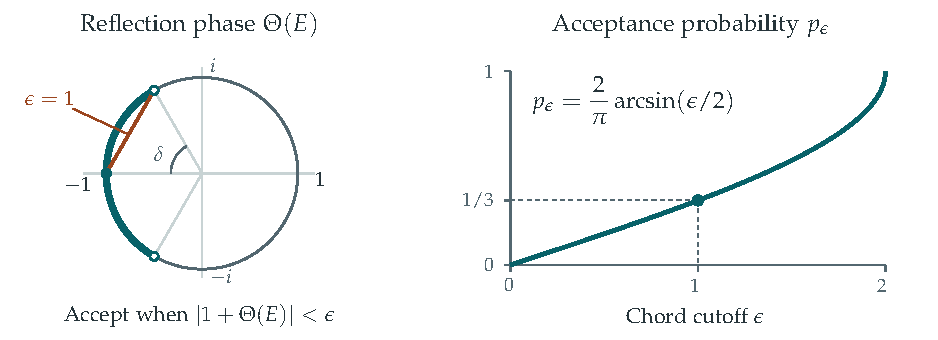
\includegraphics[width=\linewidth]{figures/manuscript/phase-window.pdf}
\caption{Postselection about the prescribed phase $-1$. At chord cutoff $\epsilon=1$ the accepted arc has angular half-width $\delta=\pi/3$, so one third of the packets are accepted on average. The curve gives the probability for any unit packet in the selected channel.}
\label{fig:phase-window}
\end{figure}

Keeping only reflections close to a given phase is a way to approximate a closed circuit while the port remains accessible. To calculate what the accepted packets measure, let $B_\alpha$ be the extension whose wall phase is $\alpha$. Disintegrating the spectral measure of $D$ by the value of $\Theta(E)$ decomposes the open response into fixed-phase resolvents~\cite{aleksandrov}. On conditioning, only phases along the accepted arc contribute, with equal angular weight,
\[
 J_\epsilon^*(D-i)^{-1}J_\epsilon
 =\frac1{2\delta}\int_{-\delta}^{\delta}
        (B_{-e^{i\theta}}-i)^{-1}\,d\theta .
\]
For $z=i$ the wall phase enters the rank-one resolvent correction through the factor $1/(\alpha-\Theta(i))$. Since $|\Theta(i)|<1$, the correction is analytic in $\alpha$ near $-1$. Its term linear in $\theta$ averages to zero on the symmetric arc, leaving an operator-norm error $O(\epsilon^2)$ relative to $(\HH-i)^{-1}$. Thus narrowing the window improves the conditional resolvent at this fixed complex frequency, at a mean cost of $1/p_\epsilon\sim\pi/\epsilon$ independent preparations per accepted packet.

\section{The shear component and its measured intensity}\label{app:weights}
\subsection*{A nonzero shear component of a theta integral}

A detector moving along a shear orbit sees an oscillation only if the wave varies on that orbit. The phase in \eqref{eq:circle} therefore requires a separate argument even for a wave of positive norm. Some output $F$ of the final integral must have a nonzero Fourier amplitude $W_cF(g_0)$ at a frequency $c\ne0$. We first use a finite-dimensional test in Alp\"oge's proof to identify a nonzero output. We then show that its overlap with a translated copy decays as the shear displacement grows. The last step connects the translation acting on the wave to the orbit sampled by the detector.

All three steps must concern the same member of the family in Alp\"oge's proof. For a primitive Dirichlet character, the source constructs a family subject to any prescribed common lower bounds. The reference space has positive rank, and at sufficiently large scales the selected input subspace maps onto it. At these scales the same selection rule supplies a real representation and a comparison map for each eligible member. The set of eligible indices is still nonempty above the common thresholds, so we fix one such index throughout~\cite{shearfamily,shearrow,shearjoin}.

Think of the reference space as a list of readouts for the theta chain. A vector of readouts, called a \emph{row}, can be compared with the chain's output because both map to the same comparison space. The embedding multiplies the norm of each row by a positive constant. For inputs with coordinates in the ground field, the chain's image there is a nonzero scalar times the embedded row. A single nonzero row therefore certifies a nonzero output. There is an input of this kind with a nonzero row. Indeed, the coordinate map has the selected input subspace in its range, and this subspace maps onto the positive-rank reference space. If every standard coordinate vector gave a zero row, their span would as well. At least one standard vector therefore detects a nonzero output of the theta chain before projection~\cite{shearrow,shearjoin}.

Write $T$ for this nonzero output in the multiplicity space at the bottom of the chain. An element of that space is a map taking a local vector to an automorphic wave. We must still connect that abstract output to a wave the detector can sample. For our chosen member, the comparison at the last step holds at every point of the output space. If the local theta map sends a test function and input $(\Phi,v)$ to $w$, the original integral in Section~\ref{sec:lift} gives $F=T(w)$. Some pair has $w\ne0$ because the local theta map is nonzero~\cite{shearjoin,shearraw}.

To see that this $w$ gives a wave of positive norm, use the Petersson inner product. It integrates one wave times the conjugate of the other over a fundamental domain with Haar measure. Rapid decay of cusp forms gives convergence. Since $T$ intertwines the irreducible local action with translations of the wave, the Petersson inner product pulled back by $T$ is a scalar multiple of the local inner product, by Schur's lemma. The scalar is positive. Pure tensors span, so $T\ne0$ has a nonzero value on at least one of them, and the Petersson norm of that value is positive. Thus for the smooth tensor $w$ produced by the integral,
\[
 \|T(w)\|_{\rm Pet}^2=\|T\|_{\rm mult}^2\,\|w\|_{\rm loc}^2>0 .
\]
Under this identification, a shear applied to $w$ translates the argument of $F$ on the \emph{right}, sending $F(g)$ to $F(g n_b)$~\cite{thetaoriginal,shearmetric}.

To compare right and left shears later, we need a shear that respects the rational symmetries of the wave. Our member of the family supplies two vectors $e,f$ over the quadratic extension, each with zero squared length but with mutual pairing one. Such a pair is called a hyperbolic pair. At the real embedding where the measurement is made, this pair gives the unitary group indefinite signature $(p,q)$~\cite{thetaoriginal,shearjoin}. The shear fixes $e$ and adds a purely imaginary multiple of $e$ to $f$. A nonzero trace-zero element of the extension supplies that multiple over the ground field. Scaling $e,f$ by $e^{t/2},e^{-t/2}$ gives a dilation that conjugates $n_b$ to $n_{e^t b}$.

The local representation belongs to the discrete series, so its matrix coefficients are square integrable~\cite{shearmetric}. One such coefficient is the overlap of a vector with its translate. Square integrability and uniform continuity under right translation together imply that this overlap tends to zero at infinity. Otherwise its magnitude would have a positive lower bound on infinitely many disjoint translates of a small neighborhood, contradicting square integrability. The Petersson identity carries this decay over to the overlap of the waves, first for finite sums of pure tensors and then by norm approximation. If every right shear fixed $F$, its overlap would instead stay at $\|F\|_{\rm Pet}^2>0$ even as $|b|\to\infty$. Thus the right action has a nonzero-frequency component of at least one sign. Dilations preserve its frequency ray, giving the translation representation used in Section~\ref{sec:line}~\cite{affine}.

The detector, however, samples $F(n_b g)$, with the shear on the \emph{left}. Suppose it saw no nonconstant Fourier component at any $g$. Fourier uniqueness on the compact shear quotient, together with continuity, would give $F(n_b g)=F(g)$ for every adelic $b$. In particular, the left shear at the real embedding used for the measurement would fix $F$. Rational changes of coordinates leave the automorphic wave unchanged. Making such a change before the shear and undoing it afterwards would therefore also leave $F$ unchanged. This gives invariance under every rational conjugate of the shear. The real components of the rational group elements are dense in $U(p,q)$. Indeed, the Cayley transform of rational skew-Hermitian matrices is dense in a neighborhood of the identity, and $U(p,q)$ is connected. Continuity now gives left invariance under $h n_b h^{-1}$ for every $h\in U(p,q)$. The group identity $(g n_b g^{-1})g=g n_b$ now explains the choice of conjugate. Since the shear acts only at the measured real place, taking $h$ to be the real component of $g$ gives precisely the right translation there. We would have $F(g n_b)=F(g)$ for every real $b$, contradicting the overlap decay. Hence some $g_0$ and $c\ne0$ give the measurable coefficient required in \eqref{eq:circle}. This existence argument determines neither its amplitude nor a preferred observation point or channel.

\subsection*{What a fixed detector measures}

Having found a frequency at which the detector responds, we can ask whether its response at the other harmonics reproduces the circle trace. Keep the observation point fixed and use the detected frequency $c$ as the unit, so $w_1>0$. The power $w_n$ in harmonic $nc$ is summed over an orthonormal basis of inputs, as in \eqref{eq:power}. Applying Parseval to successive shear derivatives gives $\sum n^k w_n<\infty$ for each $k\geq0$. In particular, the Gaussian measurement $h_w(r)=\sum_{n\geq1}w_n e^{-\pi n^2r^2}$ approaches the finite power $M=\sum_{n\geq1}w_n$ as $r\downarrow0$. The uniform count grows like $1/(2r)$ on the same scales. Equation~\eqref{eq:defect} gives the resulting failure of reciprocity even when a finite constant-mode weight is included.

We can follow the discrepancy through to the boundary response. Replacing the unweighted Gaussian sum by $h_w$ in the Mellin transform gives the pulse amplitude
\[
 A_w(z)=\tfrac12s(s-1)\pi^{-s/2}\Gamma(s/2)D_w(s),\qquad
 D_w(s)=\sum_{n\geq1}w_nn^{-s},\quad s=\tfrac12-iz.
\]
Rapid decay of the weights makes the series for $D_w$ converge locally uniformly on the whole plane. In particular, $0<D_w(1)<\infty$, so $A_w$ retains a simple zero at $s=1$. At $s=0$ the pole of $\Gamma(s/2)$ cancels the factor $s$, giving $A_w(-i/2)=-M$.

For real $E$, the measured power is $|A_w(E)|^2$. Its negative half-logarithmic derivative extends meromorphically as
\[
 B_w(z)=A_w(z)\overline{A_w(\bar z)},\qquad m_w(z)=-\frac{B_w'(z)}{2B_w(z)}.
\]
The two endpoint values above have a direct consequence for reflection. On $z=iy$, $0\leq y<1/2$, the factors of $B_w(iy)$ are the negative real amplitudes at $s=1/2\pm y$. Their product is even in $y$, remains positive up to the endpoint, and has a simple zero at $y=1/2$. Hence $m_w(iy)=\tfrac i2(d/dy)\log B_w(iy)$ starts at zero and tends to $-i\infty$ as $y\uparrow1/2$. By continuity it equals $-i$ at some positive damping. The reflection formula $(1+im_w)/(1-im_w)$ has a pole there. This conclusion concerns the phase assigned by the logarithmic-derivative prescription. Measuring harmonic power alone leaves the causal phase and stability of the detector undetermined.

The fixed detector also has too few real cancellation frequencies to reproduce the zeta spectrum. Choose $\sigma\geq2$ large enough that $\sum_{n>1}w_n n^{-\sigma}<w_1/2$. The first term gives $|D_w(\sigma+it)|\geq w_1/2$ for every $t$, while $|D_w(s)|\leq M$ throughout $\operatorname{Re}s\geq0$. Jensen's formula counts zeros in a disk by comparing the magnitude of an analytic function at its center with its size on a larger circle. Here we use concentric disks centered at $\sigma+it$ with radii $\sigma-1/4$ and $\sigma-1/8$. The smaller contains the unit segment of the critical line centered at height $t$. The larger stays in the half-plane where the bound $M$ holds. Jensen's formula therefore bounds the number of zeros on each unit segment independently of $t$. This gives $O_w(T)$ real cancellation frequencies up to $T$, whereas the simple critical-line zeros alone number $\gg T\log T$~\cite{bcy}.

The fixed detector measures correlations as well as powers. The diagonal of its correlation matrix gives the $w_n$, while the other entries measure overlaps between harmonics. In the notation of Section~\ref{sec:line}, with inner products linear in the first slot,
\[
 \sum_j W_qF_j(g_0)\overline{W_{q'}F_j(g_0)}
    =\langle T^*u_{q'},T^*u_q\rangle .
\]

Now change the detector setting when changing harmonic. The rational dilation $d(a)$ satisfies $d(a)n_bd(a)^{-1}=n_{a^2 b}$. Measuring the coefficient at $n^2c$ at the point $d(1/n)g_0$ gives $W_{n^2c}F(d(1/n)g_0)=W_cF(g_0)$ by rational automorphy and the Haar-preserving substitution $u\mapsto n^2u$. This equality holds for every input, so at zero translation the different settings repeat the same amplitude vector. Every entry of their matrix of inner products is $w_1$, and the matrix has rank one. The settings can nevertheless be distinguished by their response to translation. At setting $n$ the normalized phase is $e^{in^2\omega b}$. Averaging it over the real shear with the Poisson kernel $y/[\pi(y^2+b^2)]$ gives $e^{-n^2|\omega|y}$. At $y=\pi r^2/|\omega|$ this is the $n$th term in the circle heat trace. Assigning each setting unit weight to form the sum is a choice of measurement.

One might try to recover the uniform count by taking larger families of input waves. A related estimate in the proof concerns period maps $B_i$ with a common $D$-dimensional output space. It controls how evenly the eigenvalues of $S_{\rm per}=\sum_i c_i B_iB_i^*$, $c_i>0$, share their total weight, through the relative variance $D\Tr(S_{\rm per}^2)/(\Tr S_{\rm per})^2-1$~\cite{zhangperiods,primeguide}. One permanently blind direction and $D-1$ equally sensitive directions give a variance of just $1/(D-1)$. To infer individual harmonic powers, we would first have to identify a detector vector $v_n$ for each shear harmonic in that space. Even $S_{\rm per}=\mu I$ would give power $\mu\|v_n\|^2$. A limit yielding \eqref{eq:heatcount} would need control of each of these powers and of the high harmonics left under the Gaussian envelope.

There is also a way to approximate the uniform harmonic count with normalized wave packets on the extracted circle. The calibration and energy required can be computed explicitly. With $e_n(z)=z^n$ and $y>0$, consider
\[
 f_y=Z_y^{-1/2}\sum_{n\ge1}e^{-ny/2}e_n,\qquad
 Z_y=\sum_{n\ge1}e^{-ny}=\frac1{e^y-1}.
\]
Orthonormality gives $\|f_y\|=1$, with Born probability $e^{-ny}/Z_y$ in harmonic $n$. Multiplying the heat expectation by $Z_y$ gives
\[
 Z_y\langle e^{-\pi r^2N^2}f_y,f_y\rangle
        =\sum_{n\ge1}e^{-ny}e^{-\pi n^2 r^2}\longrightarrow h(r)
        \qquad (y\downarrow0).
\]
For each fixed $r>0$, the calibration error is at most $y\sum_{n\ge1}n e^{-\pi n^2r^2}$ since $1-e^{-ny}\le ny$. As the mode weights flatten, the calibration grows as $Z_y\sim 1/y$. The same geometric series gives the mean kinetic energy,
\[
 \langle N^2\rangle_{f_y}=\frac{1+e^{-y}}{(1-e^{-y})^2}\sim\frac{2}{y^2}.
\]
Thus these calibrated packets approach the exact trace at fixed $r$ at the cost of unbounded mean energy.

\section{Finite arithmetic data and spectral checks}\label{app:checks}

A prime power leaves two signatures in the Ramsey experiment of Section~\ref{sec:primewave}. One is local in time, a jump in slope. The other is its contribution to the full coherence for the preparation $\rho_*$. Both can be read from the smoothed prime excess $\mathcal E_\Lambda(t)$. Its ramp for the integer $n$ starts at $t=\log n$ with slope $\Lambda(n)$. Consequently $\mathcal E_\Lambda''-\mathcal E_\Lambda'+e^t$ on $t>0$ consists of point masses of weight $\log p$ at $j\log p$. Multiplying by $-e^{-t/2}$ gives the prime part of \eqref{eq:wave}.

For the full coherence, it is more useful to keep the ramps and take their Laplace transform. They contribute $-\zeta'(s)/[s(s-1)\zeta(s)]$, whose principal part at $s=1$ is canceled by the two smooth terms in $\mathcal E_\Lambda$. On inversion, a nontrivial zero $\rho$ of order $d$ contributes $d e^{\rho t}/[\rho(1-\rho)]$. The critical line is what gives these terms their quantum interpretation. The reciprocal denominator becomes $(\tfrac14+\gamma^2)^{-1}$, proportional to the probability assigned to each such eigenstate in $\rho_*$. The numerator $e^{t/2}e^{it\gamma}$ supplies the phase. The signed energies occur in pairs, so changing this phase to $e^{-it\gamma}$ leaves their sum unchanged. Together the nontrivial zeros contribute $e^{t/2}Z_*R_*(t)$.

The remaining residues are explicit. The pole at $s=0$ contributes $\log(2\pi)$, and the trivial zero at $s=-2k$ contributes $-e^{-2kt}/[2k(2k+1)]$~\cite[\S I.1, Eqs.~(I.2)--(I.4)]{primeguide}. Transferring these terms to the prime side gives \eqref{eq:primecoherence}. Both zero sums converge absolutely down to $t=0$, where $\mathcal E_\Lambda(0)=1+\gamma_{\rm E}$ and $\sum_{k\ge1}1/[2k(2k+1)]=1-\log 2$. These values give the normalization $Z_*$ and hence $R_*(0)=1$. Continuity of the ramps extends the formula to their endpoints, including each prime-power time. In Alp\"oge's proof, one-sided bounds on the growth of this same excess over large windows exclude zeros to the right of the critical line~\cite{primeinput,primeguide}.

We can also run the implication from a bounded measurement to the location of the zeros. Here $R_*$ denotes the prime expression in \eqref{eq:primecoherence}, extended evenly before assuming the critical-line property. Put $b_\rho=\rho-1/2$ and $\mathcal L R_*(q)=\int_0^\infty e^{-qt}R_*(t)\,dt$. The unconditional residue sum is $Z_*R_*(t)=\sum_\rho e^{b_\rho t}/[\rho(1-\rho)]$ for $t\ge0$, counting orders. Its weights are absolutely summable, and $|\operatorname{Re}b_\rho|<1/2$. For $\operatorname{Re}q>1/2$ we can therefore transform term by term, obtaining
\[
 Z_*(q^2-1/4)\mathcal L R_*(q)
     =q Z_*-\frac{\xi'(1/2+q)}{\xi(1/2+q)} .
\]
Indeed, dividing $q^2-1/4$ by $q-b_\rho$ gives $q+b_\rho-\rho(1-\rho)/(q-b_\rho)$. The terms linear in $b_\rho$ cancel in reflected pairs, and the paired reciprocal sum is the logarithmic derivative of the Hadamard product. If $R_*$ is bounded for all positive time, its Laplace transform is analytic throughout $\operatorname{Re}q>0$. A zero with $\operatorname{Re}\rho>1/2$ would put a pole there. Reflection then excludes zeros on the other side. In the forward direction real energies already express $R_*$ as a convex sum of phases and give $|R_*(t)|\le1$.

\subsection*{Why an upper bound can detect a growing oscillation}
\label{app:window}

An exponentially growing oscillation can be negative throughout a particular observation, and several oscillations can cancel. How, then, can an upper bound on selected intervals exclude every growing component? Write $C_\Lambda(t)$ for the prime expression $Z_*R_*(t)$ in \eqref{eq:primecoherence}, extended evenly. Before any assumption on the zeros, the explicit formula gives
\[
 C_\Lambda(t)=\sum_b c_b e^{bt},\qquad b=\rho-\tfrac12,\qquad
 c_b=\frac{d_b}{1/4-b^2},
\]
where $d_b$ is the order of the distinct zero $\rho$. The zero count gives $B=\sum_b|c_b|<\infty$, so $|C_\Lambda(t)|\le B e^{|t|/2}$. The arithmetic input is one-sided. For every $\epsilon>0$ there is a fixed $\lambda>1$ and there are arbitrarily large $U$ for which $C_\Lambda(t)\le C_\epsilon e^{\epsilon t}$ throughout $[U,\lambda U]$~\cite{primeinput,primeguide}.

The circle heat sum supplies a strictly positive averaging kernel,
\[
 k(v)=\sum_{n\ge1}e^{|v|/2-w_n}(4w_n^2-6w_n),
 \qquad w_n=\pi n^2 e^{2|v|}.
\]
By \eqref{eq:pulse} its bilateral transform $K_\theta(z)=\int k(v)e^{zv}\,dv$ is proportional to $\xi(1/2+z)$. Thus $K_\theta(b)=0$ for every term in the expansion of $C_\Lambda$. Averaging $C_\Lambda(t+v)$ against $k(v)$ gives zero at every shift $t$. In this average the positive and negative parts of the record must carry equal weight. Absolute convergence follows from $B<\infty$ and the double-exponential decay of $k$.

To isolate a possible growing component with exponent $b$ and multiplicity $d=d_b$, use a second averaging function
\[
 h_b(v)=\frac1{(d-1)!}\int_v^\infty (u-v)^{d-1}e^{b(u-v)}k(u)\,du .
\]
Its transform is $K_\theta(z)/(z-b)^d$, first by exchanging integrals for $\operatorname{Re} z>\operatorname{Re} b$, then by continuation. To justify continuation and compare the two averages, observe that $K_\theta^{(j)}(b)=0$ for $0\le j<d$. Thus the integral on the right equals minus the integral over $(-\infty,v)$ with the same integrand. This cancellation matters for a repeated zero. Dividing the transform by a single factor would leave the selected frequency invisible along with all the others. Removing its full order recovers its coefficient while keeping the new averaging function localized. Use the nearer tail on either side. For $x\to\infty$ the first harmonic gives $k(x)\asymp e^{9x/2-\pi e^{2x}}$. In the tail ratio $k(x+y)/k(x)$, the inequality $e^{2y}-1\ge2y$ for $y\ge0$ gives $|h_b(v)|/k(v)=O_b(e^{-2d|v|})$. Positivity on the intervening compact interval then gives $|h_b|\le C_b k$ everywhere.

Only the selected term survives the second average, because its transform at $b$ is $K_\theta^{(d)}(b)/d!\ne0$. Writing $C_+=\max(C_\Lambda,0)$ gives
\[
 \left|c_b\frac{K_\theta^{(d)}(b)}{d!}\right|e^{T\operatorname{Re}b}
 \le C_b\int k(v)|C_\Lambda(T+v)|\,dv
 =2C_b\int k(v)C_+(T+v)\,dv .
\]
Take $T$ at the midpoint of a good interval and $L=\tfrac12\log T$. For $|v|\le L$ the arithmetic upper bound applies for all sufficiently large $T$. The remaining tail contributes at most
$B e^{T/2}\int_{|v|>L}k(v)e^{|v|/2}\,dv
\le T^{O(1)}e^{(1/2-\pi)T}$.
The right side is consequently $O_{b,\epsilon}(e^{\epsilon T}T^{\epsilon/2})$. If $\operatorname{Re}b>0$, choosing $\epsilon<\operatorname{Re}b$ gives a contradiction along the arbitrarily late intervals. Reflection across the critical line excludes negative real parts of $b$ as well. This argument requires neither a fastest-growing mode nor any minimum spacing between frequencies.

\subsection*{Reading the scale exponent from the prime signal}\label{app:power-threshold}
Let $Y(x)$ be the bracket in \eqref{eq:primecoherence}, before multiplication by $e^{-x/2}$. How much damping makes its total power finite? Define
\[
 \sigma_c=\inf\left\{\sigma\in\mathbb R:\int_0^\infty e^{-2\sigma x}|Y(x)|^2\,dx<\infty\right\}.
\]
Unconditionally, $\sigma_c=\sup_\rho\operatorname{Re}\rho$. Indeed the explicit formula is $Y(x)=\sum_\rho e^{\rho x}/[\rho(1-\rho)]$, with absolutely summable coefficients. This gives convergence above the supremum. Conversely, finite total power at $\sigma$ makes the Laplace transform of $Y$ holomorphic for $\operatorname{Re}s>\sigma$ by Cauchy--Schwarz. The logarithmic derivative identity above gives the continued transform a pole with nonzero residue at every distinct $\rho$. Reflection gives $\sigma_c\ge1/2$, and the one-sided estimate and the positive filter of Appendix~\ref{app:window} give $\sigma_c\le1/2$. Consequently the extrema of the set of allowed amplitude decay rates, understood as infimum and supremum, are $(1-\sigma_c)/2$ and $\sigma_c/2$. This identifies them from a record defined entirely by prime powers and elementary completion terms.

At $\theta=2181/2500$, Crossley gives $8\max(0,\sigma_c-\theta)$ as the logarithmic growth exponent for the largest mass on qualifying interior runs of an ordinary-prime tent sampled at fourth powers~\cite[Proposition~11.5(c)]{crossleyquartic}.

On either occupied sign of the shear generator $Q$, dilation translates the spectral projections of $\log|Q|$. The spectral representation of this translation action~\cite{affine} gives copies of $L^2(\mathbb R,dx)$ with the Petersson norm. In one copy prepare
\[
 f_T(x)=T^{-1/2}\mathbf1_{[0,T]}(x)e^{-\sigma_c x}Y(x).
\]
This requires prime powers only through $e^T$. Dilation preserves each packet's norm. Writing $(U_h f)(x)=f(x-h)$ and taking the first slot linear gives
\[
 \lim_{T\to\infty}\langle U_h f_T,f_T\rangle
 =\sum_{\gamma\ {\rm distinct}}\frac{m_\gamma^2}{(1/4+\gamma^2)^2}e^{-i\gamma h}.
\]
Indeed $e^{-\sigma_c x}Y(x)$ has an absolutely convergent expansion in these tones. For a finite sum the expanding interval removes every cross term between distinct tones. Uniform approximation gives the displayed limit. At $h=0$ it is strictly positive, so the unaveraged total power diverges at the threshold itself. The packets tend weakly to zero because their norms on bounded intervals vanish while their full norms stay bounded. This measurement records squared amplitudes, including the square of each multiplicity. The calibrated trace in \eqref{eq:cusp-prime} counts each copy once. Each finite packet uses the native dilation and Petersson norm. Choosing its input profile from the prime count is a preparation step.

\subsection*{The moment inequalities behind the spin chain}
Could the spin chain itself prove that the zeros lie on the critical line? The point to check is the existence of a probability measure on $[0,1/u]$ with the moments $\mu_n=S_{n+1}/S_1$ computed from the primes. One can state this test entirely in terms of the thermal derivatives. Rescale the frequency to $y=u\lambda$ and write $c_n=u^n\mu_n$. On the interval $0\le y\le1$ the function $y^n(1-y)^k$ is nonnegative. Its average must therefore be nonnegative too. Expanding the power gives the explicit inequalities
\[
 \sum_{j=0}^{k}(-1)^j\binom{k}{j}c_{n+j}\ge0
 \qquad (n,k\ge0).
\]
Hausdorff's moment theorem says that these inequalities, taken together, guarantee the existence of the required probability measure~\cite{hausdorffmoments}. The first hopping amplitude used the nonnegativity of a single variance. An independent spectral proof would require a reason, from the prime data, for the whole family of inequalities.

To see how the signs constrain the zeros, let $K$ act by multiplication by $\lambda$ for the measure that the inequalities supply. Its end-site response on the right of \eqref{eq:end} is analytic at every nonreal $z$. Indeed, its denominator could vanish only if $z^2=1/\lambda-u\ge0$. We can identify the response without first assuming the zeros are real. Around $z=i\sqrt u$, dividing the right side of \eqref{eq:end} by $2z$ and expanding in $z^2+u$ gives $\sum_{n\ge0}S_{n+1}(u)(z^2+u)^n=L_\xi'(-z^2)$. By \eqref{eq:completion} this equals $-A'(z)/(2zA(z))$. Analytic continuation through the upper half-plane and reflection into the lower half-plane now exclude every nonreal pole of $-A'/A$. Each zero of $A$ produces a pole of its logarithmic derivative, so all zeros of $A$ would have to be real. Our construction used the critical-line result to establish positivity.

\subsection*{How accurately three Ramsey readings locate the change of slope}
For this calculation $R$ is the unlimited-bandwidth coherence of Section~\ref{sec:primewave}, $R_T$ is its energy-truncated version, and $\epsilon_T$ is the probability removed by that truncation.

To estimate the change in slope, measure three mean values $r_-,r_0,r_+$ at $t_0-h,t_0,t_0+h$. Choosing $0<h<\log(3/2)$ keeps the next impulse, at $\log3$, outside this window. Subtracting the slope on the left from the slope on the right gives $\widehat J_h=(r_+-2r_0+r_-)/h$. If each measured value is within $\delta$ of the mean $R_T$ at that time, the error relative to the ideal jump $J_2=\log 2/(Q\sqrt 2)$ satisfies
\[
 |\widehat J_h-J_2|
 \le h B_h+\frac{8\epsilon_T+4\delta}{h},\qquad
 B_h=\sup_{|t-t_0|\le h}|R(t)-W_{\rm reg}(t)/Q|.
\]
The choice of spacing balances two errors. Even with perfect data, this difference collects smooth curvature as well as the jump. Its weight on $R''$ is triangular, with unit height at the jump and area $h$, so the smooth contribution is bounded by $hB_h$, where $B_h\le1+\sup_{|t-t_0|\le h}|W_{\rm reg}(t)|/Q$. Reducing $h$ improves this approximation, but increases the effect of noise and of missing high-energy levels. Each sample can differ from the ideal coherence by $2\epsilon_T+\delta$, and the absolute values of the three coefficients $1,-2,1$ sum to four.

For a concrete target, spacing $h=0.05$, per-sample precision $\delta=10^{-3}$ and cutoff $T=25\,000$ suffice for a $25\%$ estimate of the first jump. The tail can be bounded from the chain response $m(z)=-A'(z)/A(z)$. For $|\gamma|>T\ge1$, $(1+\gamma^2)^{-1}\le2/(T^2+\gamma^2)$. Equation~\eqref{eq:end} then gives $Q=\operatorname{Im}m(i)$ and $\epsilon_T\le2\operatorname{Im}m(iT)/(QT)$. The logarithmic derivative in Appendix~\ref{app:boundary} gives $Q=0.046135928\ldots$ and $J_2>10.62$. Dropping the negative $\zeta'/\zeta$ term at $s=T+1/2$ gives $\epsilon_T<0.00719$. The background in \eqref{eq:wave} gives $B_h<28.1$. The resulting absolute error is below $2.64<J_2/4$.

The three mean values are themselves estimated by repeated qubit measurements. For $n$ independent shots at one time, each giving $+1$ or $-1$ with mean $R_T(t)$, Hoeffding's inequality~\cite{hoeffding} gives a probability at most $2e^{-n\delta^2/2}$ of an error larger than $\delta$. Across all three times the bound is $6e^{-n\delta^2/2}$. At $\delta=10^{-3}$, $9.6$ million shots \emph{at each time} suffice for the $25\%$ slope estimate with probability at least $95\%$. This estimate assumes that every shot can start with a fresh copy of the truncated mixture and perform the controlled evolution under $H$. How to implement those operations with the local couplings of $K$ remains open.

\subsection*{How many primes an interval requires}
A pulse of finite duration can probe the zeta energies using finitely many prime powers. To see where the cutoff enters, consider the wave trace averaged against a smooth test function $\phi$ of compact support. With $\psi_\Gamma=\Gamma'/\Gamma$, the full Weil formula, including the contribution at $t=0$, reads

\begin{align}
 W(\phi)={}&\widehat\phi(i/2)+\widehat\phi(-i/2)-(\log\pi)\phi(0)\notag\\
 &+\frac1{2\pi}\int_{\mathbb R}\widehat\phi(u)\,
             \operatorname{Re}\psi_\Gamma(1/4+iu/2)\,du\notag\\
 &-\sum_p\sum_{j\ge1}\frac{\log p}{p^{j/2}}
             [\phi(j\log p)+\phi(-j\log p)] .
 \label{eq:weil}
\end{align}
To compute the norm of a pulse $f$ confined to $(-a,a)$, choose its autocorrelation $\phi=f*\widetilde f$, where $\widetilde f(t)=\overline{f(-t)}$. In frequency space this gives the positive sum $W(\phi)=\sum_\gamma m_\gamma|\widehat f(\gamma)|^2$. In time it vanishes outside $[-2a,2a]$, so the prime sum stops at $p^j\le e^{2a}$. The two descriptions give the same norm on the interval~\cite{connesmarcolli}.

Completing the smooth pulses in this norm on the whole real line gives a Hilbert space unitarily equivalent to the scalar channel under the critical-line theorem~\cite{suzukiglobal}. On the interval, Suzuki's operator is the self-adjoint extension of differentiation with boundary phase $\pi$ in his convention. Its inverse is $H_{\rm s}^{-1}$ compressed to the interval space. Increasing $a$ admits a larger trial space, so the variational principle gives $t_{a,n}\searrow\gamma_n$ for each fixed $n$. Thus the $n$th positive interval eigenvalue $t_{a,n}$ bounds the $n$th \emph{distinct} positive ordinate $\gamma_n$ from above. A finite list of prime powers determines the inner product for this calculation, although the space of pulses on which one solves the eigenvalue problem is still infinite dimensional~\cite{suzukiconvergence}. A related finite-prime calculation illustrates the difference between this convergence theorem and numerical resolution. Andrews, Connes and La Gatta report that with primes up to $250$, the zeros of a ground-state transform agree with the first thousand zeta ordinates to more than five hundred decimal places. Reality of that transform's zeros under their simplicity and parity assumptions is a theorem. Identifying all its zeros with those of $\zeta$ at a fixed cutoff would be a stronger claim than their numerical comparison~\cite{prolate}.

For the pulse $v$ in Section~\ref{sec:primewave}, one can justify the same inner product by truncating to $[0,L]$ and smoothing. The Fourier amplitude of the truncation is $(1-e^{-(1/2+iE)L})/(1/2+iE)$. Smoothing by convolution with a unit-mass, nonnegative approximate identity gives smooth compactly supported pulses converging in the Weil norm, since $4/(1/4+E^2)$ is summable over the ordinates with multiplicity. As $L$ grows the remaining tail has norm $e^{-L/2}\sqrt{Z_*}$. Thus $\|v\|_W^2=Z_*$ and its normalized overlap with its translate is precisely \eqref{eq:primecoherence}.


\subsection*{What a finite coherence record determines}\label{app:finitecoherence}

Could an exact coherence record of duration $\tau$ tell discrete energies from a continuum? In this example the full record on $|t|\le\tau$ can also come from a normalizable packet of the free dilation, whose energies are continuous. The packet may depend on the duration. To construct one, we seek a continuous distribution of energy that gives the same overlaps as the discrete distribution over this interval.

Let $\mu$ assign each distinct signed ordinate $\gamma$ the mass $m_\gamma/[Z_*(1/4+\gamma^2)]$. In this distribution the functions $e_s(z)=e^{-isz}$ represent time shifts, with overlap $\langle e_s,e_u\rangle=R_*(s-u)$. Taking $|s|,|u|\le b=\tau/2$ gives precisely the observed range of time differences. By \eqref{eq:primecoherence}, prime powers up to $e^\tau$ therefore specify all inner products of finite sums of these functions. Complete their span in $L^2(\mu)$. The ordinates enter the following proof that the resulting space also admits a continuous energy density.

The first step is a sampling bound. Sufficiently close energy samples control a band-limited function between samples. Write $PW_L$ for the square-integrable functions on the real energy axis whose Fourier transforms are supported in $[-L,L]$. Equivalently their analytic extensions are entire functions of exponential type at most $L$. For fixed $L>0$ we claim
\[
 \|g\|_2^2\le C_L\sum_{\gamma\ {\rm distinct}}|g(\gamma)|^2 .
\]
Indeed, by the critical-line theorem the gaps between successive distinct ordinates tend to zero on both tails~\cite[Corollary~1]{goldstongap}. On a gap $[a,a+d]$, integrating the squared modulus of $g(x)=g(a)+\int_a^x g'(y)\,dy$ bounds the integral of $|g|^2$ by $2d|g(a)|^2+2d^2\int_a^{a+d}|g'|^2$. A band limit bounds the derivative by $\|g'\|_2\le L\|g\|_2$. Choose the tails far enough out that their largest gap $d$ satisfies $2d^2L^2<1/4$. If the sampling bound failed, we could find unit vectors whose sample sums tend to zero. Summing the gap estimate on both tails then forces at least half of their squared norm to stay in one fixed compact interval. Their band-limited Fourier representations give a subsequence converging locally uniformly to a nonzero entire function of type at most $L$. It vanishes at every ordinate. Jensen's formula allows only $O(r)$ zeros in $|z|\le r$, whereas shrinking gaps give superlinear growth. This proves the estimate.

The sampling bound lets us evaluate limits of time shifts at complex energies, even though the original norm measures them only at the real ordinates. Finite sums $F$ of time shifts need not decay on the real energy axis. For each compact set of complex energies choose $c>0$ large enough so the auxiliary factor $v(z)=\sin(z+ic)/(z+ic)$ has no zero there. The product $vF$ belongs to $PW_{b+1}$ and $|v(x)|^2\le C_c/(1+x^2)$ on the real axis. Sampling bounds $\|vF\|_2$ by a constant times $\|F\|_{L^2(\mu)}$. Bounded evaluation in $PW_{b+1}$ then gives locally uniform convergence for Cauchy sequences of $F$. At every atom the entire limit agrees with the limit in $L^2(\mu)$, so it represents the same vector with the same norm.

A theorem of de Branges supplies the continuous energy density once we check two symmetries of these entire functions. Conjugate reflection, $F(z)\mapsto\overline{F(\bar z)}$, preserves the space and norm. If $F$ has a zero at nonreal $w$, multiplication by $(z-\bar w)/(z-w)$ moves that zero to $\bar w$. The multiplier has modulus one on the real axis, so this operation also preserves the sampled norm. For membership, approximate $F$ by finite sums adjusted to vanish at $w$ by subtracting their values there. Their divided differences belong to the space because
\[
 \frac{e_s(z)-e_s(w)}{z-w}=-i\int_0^s e^{-i(s-u)w}e_u(z)\,du .
\]
Together with bounded point evaluation, these symmetries give the de Branges representation $\|F\|^2=\int_{\mathbb R}|F(x)/B(x)|^2\,dx$ for a structure function $B$~\cite[Theorem~23]{debrangesbook}. The weight $|1/B(x)|^2$ is the continuous energy density we sought. Its integral is one because the constant function has norm one. Thus $\psi_\tau=1/B$ is a unit packet. Pairing $e_{t/2}$ with $e_{-t/2}$ gives $\int e^{-itx}|\psi_\tau(x)|^2\,dx=R_*(t)$ throughout the interval. The density can be recovered from overlaps on the interval. Let $k$ be the vector whose inner product with $F$ returns $F(i)$. In the normalization $B(-i)=0$ the reproducing-kernel formula gives $|\psi_\tau(x)|^2=k(i)/[\pi(1+x^2)|k(x)|^2]$. Projections of $k$ onto increasing spans of exponentials at dense times in $[-b,b]$ converge in norm. Each projection uses the prime-data Gram matrix and the known values $e_s(i)=e^s$. Extending agreement to all times with one packet would equate its absolutely continuous energy measure with the atomic $\mu$, by uniqueness of Fourier transforms.

\subsection*{Computing the frequencies of a finite chain}
For a chain of $N$ sites we keep polynomials of degree at most $N-1$. There is a convenient way to compute its frequencies directly in the monomial basis. The overlap matrix is $M^{(0)}_{ij}=\mu_{i+j}$, and the Hamiltonian matrix is $M^{(1)}_{ij}=\mu_{i+j+1}$. Since the basis is nonorthogonal, the eigenvalue equation reads $M^{(1)}v=\lambda M^{(0)}v$. With $i,j\le N-1$, it uses only moments through $\mu_{2N-1}$. The largest three frequencies give estimates of the lowest three positive energies, because $E(\lambda)$ decreases as $\lambda$ increases.

We obtain these moments by expanding $L_\xi(9/4+x)$ at $x=0$ using the gamma and zeta functions at $s=2$. A coefficient $f_r$ of $x^r$ gives $S_r=(-1)^{r-1}r f_r$. Figure~\ref{fig:chain-convergence} shows the effect of adding sites. The variational calculation then ranges over a larger subspace, so the ordered Ritz frequencies increase towards the corresponding eigenvalues of $K$. Applying the decreasing function $E(\lambda)$ turns them into upper bounds on the distinct energies. These statements assume exact moments. Numerically, the sixteen-site values in Table~\ref{tab:chain} agree to the digits shown at working precisions of 200 and 260 decimal digits. Appendix~\ref{app:checks} uses moments of a Gaussian heat trace as an independent check. Its $16\times16$ matrix gives the same first three energies to six decimal places.

\subsection*{Three levels from the Gaussian}
Table~\ref{tab:chain} gives the energies obtained from thermal moments in Section~\ref{sec:chain}. The heat pulse provides an independent calculation of the same levels.

\begin{table}[!htb]
\centering
\begin{tabular}{r@{\qquad}rrr}
\hline
Sites & First energy & Second energy & Third energy \\
\hline
6  & 14.1347251871 & 21.0275131476 & 25.2969663424 \\
12 & 14.1347251417 & 21.0220396388 & 25.0108575817 \\
16 & 14.1347251417 & 21.0220396388 & 25.0108575801 \\
\hline
\end{tabular}
\caption{Positive energies inferred from the leading $N$ sites of the thermal chain at $s=2$. Figure~\ref{fig:chain-convergence} plots the errors before rounding.}
\label{tab:chain}
\end{table}

The heat calculation uses the evenness of $k$ to write its Fourier transform as $A(z)=A_2(z^2)$. Expanding the Fourier kernel, the coefficient of $y^j$ in $A_2(y)$ is $2(-1)^j\int_0^\infty x^{2j}k(x)\,dx/(2j)!$. The Taylor series then gives $\beta_j$ by the division displayed below. The paired product for $A$ identifies each coefficient with a moment of the inverse squared energies,

\begin{equation}
 -\frac{2A_2'(y)}{A_2(y)}=\sum_{j\ge0}\beta_jy^j,\qquad
 \beta_j=\sum_{\gamma>0}\frac{2m_\gamma}{\gamma^2}\,(\gamma^{-2})^j .
 \label{eq:ritz}
\end{equation}
The matrices $(\beta_{i+j})$ and $(\beta_{i+j+1})$, $0\le i,j<N$, play the same roles as the two moment matrices in the thermal chain. The first gives the inner products of monomials and the second represents multiplication by the variable, now $\gamma^{-2}$. Consequently the largest generalized eigenvalues of the second matrix relative to the first approximate the inverse squares of the \emph{lowest} energies. Taking inverse square roots at $N=16$ gives

\[
 14.134725141735,\qquad 21.022039638772,\qquad 25.010857580146.
\]
This calculation used twelve harmonics, integration up to $x=2.5$, and 180 decimal digits. Increasing these to sixteen harmonics, $x=3$ and 220 digits gave the same rounded values. A further check uses a Gaussian window $\widehat\phi(E)=e^{-E^2/20}$ in \eqref{eq:weil}, so that the first few levels dominate the spectral sum and the prime series converges absolutely. Keeping $p^j\le1000$ and $|u|\le60$ in the integral gives $9.1756700971471485\times10^{-5}$. At working precision this differs by $1.7\times10^{-20}$ from the sum of $2e^{-\gamma^2/20}$ over the three computed levels.

\subsection*{Measuring a degeneracy at the end site}
A degenerate line collects the probabilities of all its states. To see how that affects a return experiment, consider the density operator $\rho=(H_+^2+uI)^{-1}/S$ for the positive Hamiltonian with full multiplicities. Its eigenvalue $\ell_\gamma=\lambda_\gamma/S$ occurs $m_\gamma$ times and its trace is one. The end site of Section~\ref{sec:chain} therefore places total probability $m_\gamma\ell_\gamma$ on that line.

With the chain generator normalized to $K/S$, the return amplitude is $C_{K/S}(t)=\sum_{\gamma>0}m_\gamma\ell_\gamma e^{-it\ell_\gamma}$. Two features of this signal count a repeated level differently. Averaging its squared magnitude over all time leaves the square of each line's total probability, while its initial slope gives $iC_{K/S}'(0)=\operatorname{Tr}\rho^2$, the sum of the squared probabilities of the individual states. Their difference is

\[
 \lim_{\tau\to\infty}\frac1{\tau}\int_0^\tau |C_{K/S}(t)|^2\,dt-iC_{K/S}'(0)
   =\sum_{\gamma>0}m_\gamma(m_\gamma-1)\ell_\gamma^2 .
\]
It vanishes exactly when all zeros are simple. Over a finite observation time $\tau$, the interference between lines separated by $\Delta\ell$ picks up the averaging factor $\tau^{-1}\int_0^\tau e^{it\Delta\ell}\,dt$, of magnitude at most $2/(\tau|\Delta\ell|)$. Resolving such a pair by time averaging therefore calls for $\tau|\Delta\ell|\gg1$. The lines accumulate at zero, so no finite observation time resolves every pair.

Counting states with
multiplicity, the Riemann--von Mangoldt law gives
$\ell_n\asymp(\log n)^2/n^2$ as $n\to\infty$. Hence $\rho$ has finite
von Neumann entropy, and $\operatorname{Tr}\rho^\alpha$ is finite exactly
for $\alpha>1/2$ among positive $\alpha$.

\subsection*{Prime filters and return times}
At a prime time $\log p$, the arithmetic filter has a simple action on the scale record. For a rapidly decreasing probe $f$, let $x$ be the logarithm of the resolution and write $h_f(x)=e^{x/2}\sum_{n\ge1}f(ne^x)$. The terms with indices $n=pm$ alone contribute $p^{-1/2}h_f(x+\log p)$. Thus a shift by $\log p$ isolates every $p$th harmonic. Figure~\ref{fig:prime-filter} shows this for $p=2$. Subtracting those harmonics acts on the scale record and on the associated quantum packet as

\begin{equation}
 h_f(x)\longmapsto h_f(x)-p^{-1/2}h_f(x+\log p),\qquad
 \mathcal S_p=I-p^{-1/2}e^{i(\log p)H}.
 \label{eq:sieve}
\end{equation}
Here a quantum packet is a limit of smooth time signals in the arithmetic norm of Appendix~\ref{app:checks}. The shift in the first expression acts on each energy component of the packet by a phase, giving the exponential in the second~\cite{suzukiglobal}.

\begin{figure}[!htb]
\centering
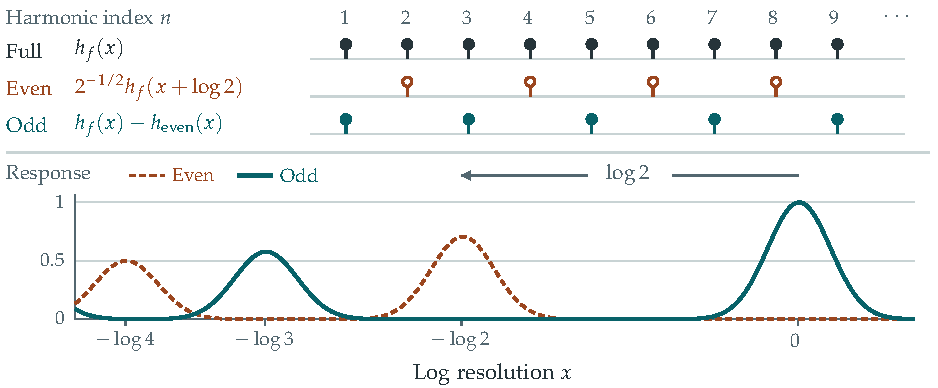
\includegraphics[width=\linewidth]{figures/manuscript/prime-filter.pdf}
\caption{The prime-two filter for $f(u)=\exp[-(\log u)^2/(2\sigma^2)]$, $u>0$, with $\sigma=0.065$. The dashed even contribution is the full scale record shifted left by $\log 2$ and scaled by $1/\sqrt2$. Subtracting it from the full record leaves the solid odd contribution.}
\label{fig:prime-filter}
\end{figure}


Meyer's construction identifies signals differing by an element in the range of arithmetic summation. Translation preserves that range, so the same filter acts on his quotient space~\cite{meyerphysics}. Knowing $\mathcal S_p$ then determines the time-step operator $e^{i(\log p)H}$. Two primes already supply the continuous evolution. Since $\log2/\log3$ is irrational, integer combinations of their two time steps are dense, and strong continuity determines $e^{-itH}$ at every time. These evolution operators distinguish energies and act as scalars within each degenerate level.

The same time interval has a geometric meaning for the shear frequencies. For the shear character of Section~\ref{sec:lift}, consider all its rational multiples with denominators a power of $p$. The real frequencies are $\omega\mathbb Z[1/p]$. Dilation by $e^t$ preserves this entire set precisely when $e^t$ and $e^{-t}$ both belong to $\mathbb Z[1/p]$. Its positive invertible elements are $p^j$ for $j\in\mathbb Z$, so $\log p$ is its least positive return time~\cite{knots}. One can ask separately whether the Ramsey interference revives at that time, and whether the observed point returns to its starting position.

For the Ramsey coherence, equality $|R(t)|=1$ requires every occupied phase $e^{-it\gamma}$ to agree. At $t\ne0$ all signed zeros would then lie on one arithmetic progression. Such a progression has only $O(T)$ points to height $T$, fewer than the simple zeros alone~\cite{bcy}. Hence $|R(t)|<1$ for every nonzero time. Arbitrarily accurate recurrences of the coherence still occur. Any finite set of phases returns simultaneously as close to one as desired at arbitrarily large times, and absolute convergence makes the weight of the omitted phases arbitrarily small. Throughout, the density operator $\rho_R$ stays stationary.

At a fixed automorphic level a returning point at $t=\log p$ would require a rational group element with marked eigenvalue $e^{t/2}$ and finite components conjugate into compact groups. Bounded positive and negative powers at the finite places make the eigenvalue an algebraic unit. Its square $p$ rules this out.

The function-field analogue illustrates how much a single time step can reveal. For a smooth projective curve over $\mathbf F_q$, the eigenvalues of Frobenius on degree-one cohomology have modulus $\sqrt q$. After division by $\sqrt q$ their phases admit a unitary realization with time step $\log q$. One such step determines energies only modulo $2\pi/\log q$. This single-step ambiguity explains why the two incommensurate prime times in this appendix suffice to distinguish energies.


\section{From Petersson waves to modular resonances}\label{app:resonance}

\subsection*{What survives every step of the theta lift}\label{app:cut-period}
An input at the top of a finite chain of theta integrals produces a wave at the bottom. We can calculate its amplitude at a detector by passing the input partway down the chain and passing the detector back up to meet it. How far each travels is immaterial. Write $T_j:H_{j+1}\to H_j$ for the actual downward maps on the fixed-level spaces of the chain, equipped with their Petersson inner products. The upward maps are their adjoints~\cite{stagebasis,shearraw}. Take an input $x_m=x$ and a detector $y_0=y$, and propagate them by $x_j=T_jx_{j+1}$ and $y_{j+1}=T_j^*y_j$. At every cut,
\[
       \langle x_j,y_j\rangle_j
       =\langle x_{j+1},y_{j+1}\rangle_{j+1}.
\]
Thus even the phase of the detected amplitude is independent of where we cut the chain.

Summing its squared magnitude over an orthonormal basis of bottom detectors gives a positive quantity. With $C_0=I$ and $C_j=T_0\cdots T_{j-1}$, Parseval's identity gives $\|C_jx_j\|_0^2$. The forms $G_j=C_j^*C_j$ are positive semidefinite and are uniquely determined by $G_0=I$ and $G_{j+1}=T_j^*G_jT_j$. Their meaning follows by identifying waves that give the same bottom output. In this quotient the map $[v]\mapsto C_jv$ is an isometry onto the image of $C_j$ with its bottom Petersson norm. Under these identifications a downward step includes one image in the next, with the measured output unchanged. An individual link gives a related isometry. On a nonzero fixed Hecke and type component where the inner-product formula gives $TT^*=\ell I$, the rescaled upward map $T^*/\sqrt{\ell}$ preserves the Petersson norm. The positive scalar $\ell$ belongs to that component and to the chosen link~\cite{stagebasis}.

For rational input coordinates satisfying the period comparison, the lift also gives an algebraic constraint. After the prescribed changes of coordinates and multiplication by the period factor, a Petersson overlap equals the marked complex embedding of a number $b$ in the coefficient field $K$~\cite{shearrow}. For a nonzero such $b$, the number-field product formula gives
\[
 \sum_{\sigma:K\hookrightarrow\mathbb C}\log|\sigma(b)|
   =\sum_{P}\operatorname{ord}_{P}(b)\log (N P) .
\]
The sum counts both complex conjugate embeddings. On the right, $P$ runs over nonzero prime ideals, and $N P$ is the size of the residue field. For an integral period, every additional prime divisor raises the minimum possible product of those complex sizes. Bounding those sizes across the family requires the norm and lattice estimates of the proof~\cite{primeguide}. The index $j$ moves the cut through one fixed composite. The cusp time $\tau$ advances a wave on a surface. One can multiply a link by any nonzero scalar and its adjoint by the conjugate scalar and both measurements still agree at every cut. It is the arithmetic estimate on the size of the links that constrains a resonance lifetime.

\subsection*{What a fixed wave can retain}
The Petersson inner product measures the overlap of two automorphic waves by integrating over a fundamental domain. At the stage used in Section~\ref{sec:cusp}, this overlap factors into an inner product of multiplicity vectors and an inner product of vectors in the local representations. The real motion acts on the latter. At the marked place its representation $\pi$ belongs to the discrete series. Schur orthogonality therefore embeds its Hilbert space isometrically into $L^2(G)$ for $G=U(p,q)$. For a fixed unit vector $w$, the embedding sends $v$ to $g\mapsto\sqrt{d_\pi}\langle \pi(g)v,w\rangle$, where $d_\pi$ is the formal degree and the first slot is linear. Acting on $v$ becomes right translation of the coefficient~\cite{thetaoriginal,shearmetric}.

The dilation subgroup $A=\{a_t\}$ is a closed copy of $\mathbb R$. On the marked hyperbolic pair its two scale factors are $e^{t/2}$ and $e^{-t/2}$, so $a_t$ escapes every compact set as $|t|$ grows. Decomposing Haar measure along the cosets $gA$ expresses right translation by $a_t$ as ordinary translation on copies of $L^2(\mathbb R)$. Fourier transformation along each copy gives an integrable spectral density for the overlap of any two finite-norm vectors, by Cauchy--Schwarz. Its Fourier transform tends to zero. The Petersson factorization carries this conclusion to the whole fixed-stage sector, including superpositions of its multiplicity vectors. A fixed bounded linear pickup thus loses its signal at late times, even though the total Petersson norm is conserved. The same restriction argument for the closed shear subgroup gives $\ker Q=0$ for its generator $Q$. In fact any unitary step satisfying $U^*QU=pQ$ permutes the spectral bands of $|Q|$ in Section~\ref{sec:lift}. They exhaust the whole space. Each is a translate of the central band, so $U$ is a bilateral shift with multiplicity and has no eigenvectors. This stronger conclusion also covers an interaction that preserves the stated rescaling. We can test the information in the conserved Petersson norm on a single translation coordinate $x$. For any $a>0$ the unit packet $v_a(x)=\sqrt{2a}\,e^{-a x}\mathbf1_{[0,\infty)}(x)$ has overlap $\langle U_t v_a,v_a\rangle=e^{-a|t|}$ with its translate. The dilation and its norm are exactly the same at every $a$. The measured rate changes with the packet. This example concerns overlaps on a shear ray. Arithmetic resonances are identified by the distinct scattering experiment below.

\subsection*{A nonzero source on the modular surface}
Alp\"oge's pair $e,f$ consists of vectors over the CM field $K$, with zero self-pairings and $\langle e,f\rangle=1$. The selected stage supplies at least one pair~\cite{thetaoriginal,shearjoin}. For any nonzero $\delta\in K$ with $\bar\delta=-\delta$, the map
\[
  \iota\!\begin{pmatrix}a&b\\c&d\end{pmatrix}
   =\begin{pmatrix}a&\delta b\\c/\delta&d\end{pmatrix},
   \qquad a,b,c,d\in\mathbb Q,\quad ad-bc=1,
\]
preserves the off-diagonal Hermitian form on their plane. Extending by the identity on its orthogonal complement gives a rational subgroup. Its real action $\iota_\infty$ is diagonal across the infinite places. This specifies a different motion from a dilation supported at the marked place alone.

Choose $g_0$ with $F(g_0)\ne0$ for a smooth theta output $F$, and restrict it to $h\mapsto F(\iota_\infty(h)g_0)$. At the finite places $F$ has an open right stabilizer. The preimage under $\iota$ of its conjugate by the finite component of $g_0$ contains a principal congruence subgroup of $\mathrm{SL}_2(\widehat{\mathbb Z})$. Left rational invariance therefore makes the restriction invariant under some $\Gamma(N)$. To descend to the modular surface, average the squared modulus over right rotations and sum over the finitely many sheets above level one. Continuity and the nonzero value at $h=1$ give a strictly positive average at its image. A smooth nonnegative aperture positive at that point, with compact support, gives a compactly supported source $f_0\ge0$ of positive integral.

For real $s>1$, each summand of the Eisenstein wave $E(z,s)$ is positive, so $P(s)=\int f_0(z)E(z,s)\,d\mu(z)>0$. Compact support gives meromorphic continuation of this pairing. Its zeros on the scattering line are isolated, and the continuous spectral transform of $f_0$ is consequently nonzero almost everywhere. This one cusp has one scattering channel. The functional equation $P(s)=\phi(s)P(1-s)$ recovers its response from the two amplitudes as a meromorphic quotient~\cite{muellerspec}. Intensity detection and propagation on the surface are operations specified by the probe.

\subsection*{Energy and interference at the cusp}\label{app:outgoing-flux}
Uetake represents the reduced scattering space by a subspace $K_c$ of $L^2(-\infty,0)$. In the outgoing coordinate $x$, time evolution translates a profile to the right and discards the portion past the exit. The truncated translation preserves $K_c$, so its restriction already gives the reduced semigroup $S(\tau)$~\cite[Theorems~4.4 and~5.1]{uetake}. For a smooth profile $h$ and $\tau\ge0$ the surviving field is $(S(\tau)h)(x)=h(x-\tau)$. Hence
\[
 \|S(\tau)h\|_2^2=\int_{-\infty}^{-\tau}|h(x)|^2\,dx,\qquad
 \frac{d}{d\tau}\|S(\tau)h\|_2^2=-|h(-\tau)|^2 .
\]
All the outgoing flux passes through one scalar amplitude. A mode of generator eigenvalue $-\rho/2$ solves $-h'=-\rho h/2$. Setting $h_\rho(0)=1$ gives $h_\rho(x)=e^{\rho x/2}$ and $\|h_\rho\|_2^2=1/\operatorname{Re}\rho$. Thus the balance law reads off each width from the ratio of exit flux to remaining squared norm. For two distinct modes the difference $h_{\rho_1}-h_{\rho_2}$ has positive norm and zero initial flux. Even when both modes lie on the critical line, compensating their amplitudes by $e^{\tau/4}$ makes the squared norm of their difference initially increase.

Could a different calibration of the same wave norm restore conservation? At a critical height $\gamma$, write $u_\gamma=2^{-1/2}h_{1/2+i\gamma}$ for the unit profile. Direct integration gives
\[
 |\langle u_\gamma,u_\eta\rangle|=(1+(\gamma-\eta)^2)^{-1/2}.
\]
Distinct simple critical heights come arbitrarily close. Indeed, a positive proportion of the zeros up to $T$ are simple and on the line~\cite[Theorem~1.1]{bcy}, and their number therefore grows faster than $T$. Along close pairs a constant phase can make the difference of the two unit profiles tend to zero in outgoing norm. In any conserved inner product for $e^{\tau/4}S(\tau)$ the two modes must be orthogonal, since their relative phase changes with time. If the new norm were bounded above and below by fixed positive multiples of the outgoing norm, their difference would tend to zero while its squared norm stayed bounded away from zero. This rules out such a calibration even on the span of the known simple critical modes. On a full generalized eigenspace a positive conserved norm would also forbid Jordan growth. Since the scalar differential equation supplies just one eigenvector direction per zero, this stronger demand would imply simplicity. The time average on successive growth quotients below accommodates repeated zeros.

There is a direct consequence for a pulse observed over any prescribed duration $T$. For this computation write $v=-x\geq0$, so in the reflected coordinate the reduced evolution is $(S(t)f)(v)=f(v+t)$~\cite[Theorem~5.1]{uetake}. The fraction retained therefore decreases with $t$. We claim $\|S(T)\|=1$ even on the closed span of simple critical-line modes. Indeed, if each interval of some fixed width contained at most $k$ simple critical heights, their count up to $Y$ would be $O(Y)$. Thus for each $k$ we can choose $k+1$ such ordinates in intervals of arbitrarily small width.

Take the order-$k$ divided difference in $\gamma$ of their profiles $e^{-v/4-i\gamma v/2}$. Removing the first tone's phase preserves every tail norm. As the cluster shrinks, the simplex integral for divided differences gives a pointwise limit proportional to $v^k e^{-v/4}$ and an absolute bound $v^k e^{-v/4}/(2^kk!)$. Thus convergence holds in $L^2$. The limiting fraction of squared norm retained at $T$ is
\[
 \frac{\int_T^\infty v^{2k}e^{-v/2}\,dv}{\int_0^\infty v^{2k}e^{-v/2}\,dv}
 =e^{-T/2}\sum_{j=0}^{2k}\frac{(T/2)^j}{j!}\xrightarrow[k\to\infty]{} 1 .
\]
At $T=4$, for example, three coalescing tones ($k=2$) retain a fraction approaching $7e^{-2}$ of the squared norm, while any of the three alone retains $e^{-2}$. Since even the finite packets can approach the displayed limit and loss is monotone, there are unit packets that retain any prescribed fraction less than one throughout $[0,T]$. For every fixed packet, the tail integral tends to zero as $T\to\infty$.

For the finite example in Section~\ref{sec:cusp}, take consecutive positive heights $\gamma_j\simeq 430.32874543,431.30130693,432.13864173$. In the original coordinate $x<0$ let $b_j=(1/2+i\gamma_j)/2$, $h(x)=\sum_{j=1}^3 a_j e^{b_jx}$ and
\[
 a_j=\frac{e^{i\gamma_j}}{\prod_{k\ne j}(\gamma_j-\gamma_k)},\qquad
 \|S(T)h\|_2^2=\sum_{j,k=1}^3
 \frac{a_j\overline{a_k}\, e^{-(b_j+\overline{b_k})T}}{b_j+\overline{b_k}} .
\]
The coefficients make the exit amplitude and its first derivative vanish at the midpoint $T=2$, since the second divided difference of either a constant or a linear function is zero. At $T=4$ the retained fraction of the initial squared norm is $0.85750985011732\ldots$. The counting argument allows arbitrarily long observation times, at the cost of choosing new modes and controlling their phases.

\subsection*{The conserved modal energy}
For the nonnegative hyperbolic Laplacian, Uetake's outgoing generator $A_c$ has eigenvalues $-\rho/2$ with the orders of the zeros as algebraic multiplicities~\cite{uetake}. In the time convention $t=\tau/2$, the compensated generator $B=2A_c+\tfrac12 I$ therefore has eigenvalues $-i\gamma$ on the critical line. Consider the vectors whose continuous forward orbit has finite-dimensional linear span. On each such span the matrix exponential extends uniquely to all real times. This description uses the generator without specifying a list of zeros. Denote by $V_k$ the vectors whose compensated evolution grows at most as $(1+|t|)^k$ in both directions, and put $V_{-1}=0$. Any off-line exponent is excluded by this two-sided growth condition. The arithmetic bound is what ensures that every nontrivial zero is retained. For $x\in V_k$ the leading polynomial coefficient determines the time-averaged energy
\[
 \lim_{T\to\infty}\frac{1}{T^{2k+1}}\int_0^T\|e^{tB}x\|^2\,dt
 =\frac{1}{(2k+1)(k!)^2}\sum_\gamma
          \|(B+i\gamma I)^k x_\gamma\|^2 .
\]
Here $x_\gamma$ is the component in the generalized eigenspace at $-i\gamma$. Cross terms between different frequencies vanish in the limit. The kernel is precisely $V_{k-1}$. On each quotient a time shift preserves the resulting norm, and a Jordan block of length $d$ contributes one dimension in each of $d$ successive quotients.

Completing the orthogonal sum of the quotients gives a self-adjoint generator $H_{\rm mod}$ with the recorded multiplicities. For $D_*=(\tfrac12+iH_{\rm mod})^{-1}$, zero counting gives $\Tr(D_*^*D_*)<\infty$. The prime ramp in \eqref{eq:primecoherence} assigns exactly the weight $(\tfrac14+\gamma^2)^{-1}$ to each copy. Thus $C_\Lambda(t):=Z_*R_*(t)=\Tr(D_*^*D_* e^{-itH_{\rm mod}})$, and pulses of strengths $a_j$ at times $t_j$ have stored energy
\[
 \frac12\sum_{j,k}\bar a_j a_k C_\Lambda(t_k-t_j)
 =\frac12\left\|\sum_j a_j e^{-it_jH_{\rm mod}}D_*\right\|_{\rm HS}^2 .
\]
The squared Hilbert--Schmidt norm sums over all orthonormal input modes. A common time shift acts unitarily on their outputs and preserves this energy. For two opposite unit pulses separated by $\log 6$, the stored work is $C_\Lambda(0)-C_\Lambda(\log 6)=0.0327614132\ldots$. Only the prime powers $2,3,4,5$ have nonzero ramp weights in this calculation.

The work interpretation can be checked for a smooth drive $u$ of compact support. Its output is $y(t)=\int_{-\infty}^t C_\Lambda(t-r)u(r)\,dr$. Replacing the pulse sum in the energy by its double integral and differentiating the two endpoints gives $\dot{\mathcal W}(t)=\operatorname{Re}[\overline{u(t)}y(t)]$. The energy is constant after switch-off. Here the work is calibrated against the collective response of \eqref{eq:cusp-prime}.

\subsection*{Truncating the reconstruction from cusp data}
Let $w=\tfrac12-iz$, $d(w)=C'(w/2)/[2C(w/2)]$ and $a(v)=1/v+1/(v-1)-\tfrac12\log\pi+\tfrac12(\Gamma'/\Gamma)(v/2)$. The finite estimate $i[a(w+N)+\sum_{j=0}^{N-1}d(w+j)]$ differs from $m(z)$ by the endpoint $i(\zeta'/\zeta)(w+N)$ (target minus estimate). Its magnitude is at most $\sum_{n\ge2}(\log n)n^{-\sigma}$ for $\sigma=\operatorname{Re}w+N>1$. At the three damped frequencies in Section~\ref{sec:cusp}, $\sigma=33.5$ for $N=32$. The first term and the integral from 2 to infinity bound that sum by $6.08\times10^{-11}$. For the numerical comparison we used Euler-transformed alternating integer sums for the cusp slopes and independently integrated the pulse $k$ and its first logarithmic moment from \eqref{eq:pulse}.

\section{Eleven resonators over a damped frequency band}\label{app:circuit}
How could we check the accuracy of the circuit at frequencies between the points used in the calculation? Figure~\ref{fig:resonators} shows eleven resonator branches in parallel at the terminals. In each branch the printed frequency and strength in Table~\ref{tab:resonators} specify the component values $L_j=1/d_j$ and $C_j=d_j/\omega_j^2$. These numbers come from the prime gas at inverse temperature two. To bound the reflection error over the entire band, we combine a sweep at discrete frequencies with an analytic bound on how far the response can bend between samples.

\begin{table}[!htb]
\centering
\begin{tabular}{r@{\quad}rr@{\qquad\qquad}r@{\quad}rr}
\hline
$j$ & $\omega_j$ & $d_j$ & $j$ & $\omega_j$ & $d_j$\\
\hline
1 &14.134725 &2         &7  &44.235239 &4.941255\\
2 &21.022040 &2         &8  &55.219053 &10.104389\\
3 &25.010858 &2.0000004 &9  &76.186131 &23.774624\\
4 &30.426365 &2.0055759 &10 &127.55057 &84.042042\\
5 &32.966704 &2.0359943 &11 &417.53930 &1275.5029\\
6 &38.229004 &2.9518674 & & &\\
\hline
\end{tabular}
\caption{Branch frequencies $\omega_j$ and strengths $d_j$ for the circuit in Figure~\ref{fig:resonators}. Values are in the normalized units of \eqref{eq:branches}.}
\label{tab:resonators}
\end{table}

The couplings near two have a spectral interpretation. For a branch whose frequency and end-site weight converge to $\gamma$ and $w_\gamma$, respectively, \eqref{eq:branches} gives $d_j\to2S w_\gamma/\lambda_\gamma=2m_\gamma$. The first three values, $2$, $2$ and $2.0000004$, are consistent with simple zeros. Certifying a multiplicity this way would require isolating the line and bounding the error in its inferred order. At higher frequencies a branch can represent the combined response of several levels. The uniform error estimate below applies to the reflection at the port.

\subsection*{From thermal moments to component values}
The chain calculation gives moments, while building a resonator requires two numbers, its frequency and its strength. The conversion is easier numerically if we rescale the chain variable to $X=200\lambda$. Its end-site moments $M_k=200^k\mu_k$ are determined by the Taylor coefficients of $L_\xi$ in \eqref{eq:powers},
\[
 M_k=\frac{(-1)^k(k+1)}{200S}[t^{k+1}]L_\xi(u+200t),\qquad u=9/4.
\]
An $N$-branch circuit requires the moments $M_0$ through $M_{2N-1}$. They determine the monic polynomial $p_N(X)=X^N+\sum_{j<N}a_j X^j$ orthogonal to $1,X,\ldots,X^{N-1}$ through the equations $\sum_{j<N}M_{i+j}a_j=-M_{i+N}$ for $0\le i<N$. Its roots $x_j$ give the eigenvalues of the compressed chain. Indeed, after multiplication by $X$, taking the remainder modulo $p_N$ discards exactly the component orthogonal to the retained sites.

Returning to the original units gives $\lambda_j=x_j/200$. The first $N$ moments then determine the end-site probabilities through $\sum_j\nu_j x_j^k=M_k$ for $0\le k<N$. Substitution in \eqref{eq:branches} gives the circuit parameters. We solved the moment equations and isolated the roots with 768-bit ball arithmetic (Arb via python-flint 0.9.0) before rounding the parameters to the table.

\subsection*{Why the error bound holds between sample frequencies}
Let $f(z)=\Theta(z)-\widehat\Theta_{11}(z)$ be the reflection error for the printed parameters. Damping places the measurement line $z=E+i$ inside the region where both reflections are analytic and bounded by one. For the circuit, passivity gives the bound because positive $L_j,C_j$ give $Y_N$ nonnegative real part for $\operatorname{Re}\sigma>0$. For the exact reflection the bound follows from \eqref{eq:theta}. Hence $|f|\le2$ throughout the upper half-plane. A disk of radius $r<1$ centered on the measurement line stays in this region. Cauchy's estimate gives $|f''(E+i)|\le 4/r^2$, and allowing $r$ to approach one gives $|f''|\le4$ on the band.

For a grid of spacing $h$, the difference between $f$ and its linear interpolation is at most $h^2\sup |f''|/8$. This familiar interpolation estimate applies also to complex amplitudes, since the error is the integral of the second derivative against the interpolation error kernel.

The sweep uses the 2001 points $z_k=10+k/100+i$, $0\le k\le2000$. At each point the logarithmic derivative in Appendix~\ref{app:boundary} gives $m=i\xi'(s)/\xi(s)$ at $s=1/2-iz_k$, while \eqref{eq:branches} gives the circuit response at $\sigma=-iz_k$. At 160-bit ball precision the largest upper bound on $|f(z_k)|$ is less than $1.760\times10^{-4}$. The line segment between two sampled complex amplitudes stays within the larger of their two moduli. Adding the interpolation allowance $5\times10^{-5}$ for $h=0.01$ therefore gives

\[
 \sup_{10\le E\le30}|\Theta(E+i)-\widehat\Theta_{11}(E+i)|
 <2.26\times10^{-4}.
\]
The bound includes the rounding of the printed parameters and assumes ideal inductors and capacitors. A single frequency is enough to rule out a proposed design for this band. At $30+i$ every exact truncation with $1\le N\le10$ has error greater than $2.39\times10^{-3}$, with the smallest of these errors at $N=10$. Eleven is therefore the first truncation of this chain that meets the tolerance of $10^{-3}$ across the band. The minimum for other network designs could differ.

\begingroup\small
\begin{thebibliography}{99}
\setlength{\itemsep}{0.75pt}\setlength{\parsep}{0pt}\setlength{\parskip}{0pt}
\addcontentsline{toc}{section}{\refname}
\bibitem{polya} G. P\'olya, letter to A. Odlyzko, 3 January 1982.
\href{https://www-users.cse.umn.edu/~odlyzko/polya/index.html}{Correspondence on the origins of the Hilbert--P\'olya conjecture}.

\bibitem{alpoge} L. Alp\"oge, \href{https://alpo.ge/remark.pdf}{\emph{Remark}}, announcement, 20 November 2026.

\bibitem{sutherland} Lean and Mathlib communities, \href{https://leanprover-community.github.io/blog/posts/riemann-hypothesis/}{\emph{Lean verification of the Riemann Hypothesis}}, 21 November 2026.
A.~V. Sutherland, \href{https://math.mit.edu/~drew/grh/}{\emph{Verification files for the Lean proof of the Riemann Hypothesis}}, including the source archive checksum and independent verification records.

\bibitem{primeinput} L. Alp\"oge, same release, \href{https://github.com/TomasOrtega/RH/blob/a6ac91a412dcbaab31801355ec5707024a71bf65/extracted/lean/src/Development/AutomorphicArithmetic/DedekindLFunctions/LandauTheorems/ChBalance.lean\#L200-L209}{character-family balance} and \href{https://github.com/TomasOrtega/RH/blob/a6ac91a412dcbaab31801355ec5707024a71bf65/extracted/lean/src/Formalism/SizeWindowBrackets/GrowthBoundGivesRiemannHypothesis.lean\#L109-L121}{window bounds entering the critical-line argument}.

\bibitem{weilcurves} A. Weil, \href{https://doi.org/10.1073/pnas.27.7.345}{\emph{On the Riemann hypothesis in function-fields}}, Proc. Natl. Acad. Sci. USA 27 (1941), 345--347.

\bibitem{deligne} P. Deligne, \href{https://www.numdam.org/articles/10.1007/BF02684373/}{\emph{La conjecture de Weil I}}, Publ. Math. IH\'ES 43 (1974), 273--307.

\bibitem{selberg} A. Selberg, \href{https://mathweb.tifr.res.in/Documents/Publications/Studies/Zeta_Functions.pdf}{\emph{Harmonic analysis and discontinuous groups in weakly symmetric Riemannian spaces with applications to Dirichlet series}}, reprinted in TIFR, \emph{Zeta Functions}.

\bibitem{uetake} Y. Uetake, \href{https://doi.org/10.4064/ap92-2-1}{\emph{The Lax--Phillips infinitesimal generator and the scattering matrix for automorphic functions}}, Ann. Polon. Math. \textbf{92} (2007), 99--122, especially Theorems~4.4 and~5.1.

\bibitem{muellerspec} W. M\"uller, \href{https://www.math.uni-bonn.de/people/mueller/skripte/specauto.pdf}{\emph{Spectral theory of automorphic forms}}, lecture notes (2010), \S\S2.3--2.6.

\bibitem{montgomery} H. L. Montgomery, \href{https://public.websites.umich.edu/hlm/paircor1.pdf}{\emph{The pair correlation of zeros of the zeta function}}, Proc. Sympos. Pure Math. 24 (1973), 181--193.

\bibitem{odlyzko} A. M. Odlyzko, \href{https://www-users.cse.umn.edu/~odlyzko/doc/arch/zeta.zero.spacing.pdf}{\emph{On the distribution of spacings between zeros of the zeta function}}, Math. Comp. 48 (1987), 273--308.

\bibitem{berry} M. V. Berry and J. P. Keating, \href{https://michaelberryphysics.wordpress.com/wp-content/uploads/2013/06/berry307.pdf}{\emph{The Riemann zeros and eigenvalue asymptotics}}, SIAM Rev. 41 (1999), 236--266.

\bibitem{connes} A. Connes, \href{https://arxiv.org/abs/math/9811068}{\emph{Trace formula in noncommutative geometry and the zeros of the Riemann zeta function}}, Selecta Math. 5 (1999), 29--106.

\bibitem{weilcriterion} A. Weil, \href{https://denisevellachemla.eu/transc-Weil-1952.pdf}{\emph{Sur les formules explicites de la th\'eorie des nombres premiers}}, Medd. Lunds Univ. Mat. Sem., volume dedicated to M. Riesz (1952), 252--265.

\bibitem{zagier} D. Zagier, \href{https://people.mpim-bonn.mpg.de/zagier/files/scanned/EisensteinRiemannZeta/fulltext.pdf}{\emph{Eisenstein series and the Riemann zeta function}}, in \emph{Automorphic Forms, Representation Theory and Arithmetic} (1981), p.~276 and \S4.

\bibitem{conreyli} J. B. Conrey and X.-J. Li, \href{https://arxiv.org/abs/math/9812166}{\emph{A note on some positivity conditions related to zeta- and $L$-functions}}, Int. Math. Res. Not. (2000), 929--940.

\bibitem{meyerphysics} R. Meyer,
\href{https://arxiv.org/abs/math/0412277}{\emph{A spectral interpretation for the zeros of the Riemann zeta function}},
Theorems~3.3, 4.1, 5.8 and Corollary~4.2.

\bibitem{suzukiglobal} M. Suzuki,
\href{https://arxiv.org/html/2301.00421v3}{\emph{On the Hilbert space derived from the Weil distribution}}, \S\S2, 4.1 and~6.

\bibitem{jacobi} G. Teschl, \href{https://www.mat.univie.ac.at/~gerald/ftp/book-jac/}{\emph{Jacobi Operators and Completely Integrable Nonlinear Lattices}}, Amer. Math. Soc., Providence, RI, 2000, Ch.~2.

\bibitem{connesmarcolli} A. Connes and M. Marcolli, \href{https://alainconnes.org/wp-content/uploads/bookwebfinal-2.pdf}{\emph{Noncommutative Geometry, Quantum Fields and Motives}},
Amer. Math. Soc., Providence, RI, 2008, Ch.~2, \S2.

\bibitem{suzukiconvergence} M. Suzuki,
\href{https://arxiv.org/html/2610.32704v1}{\emph{Spectral convergence associated with Weil's quadratic form}}, arXiv:2610.32704 (2026), Theorems~1.1 and~3.3 and Proposition~6.1.

\bibitem{thetaoriginal} L. Alp\"oge, released Lean source, \href{https://github.com/TomasOrtega/RH/blob/a6ac91a412dcbaab31801355ec5707024a71bf65/extracted/lean/src/Formalism/LocalToGlobal/IndefiniteReal/OrthogonalComplementCharacterisation.lean\#L44-L55}{the last theta integral}, \href{https://github.com/TomasOrtega/RH/blob/a6ac91a412dcbaab31801355ec5707024a71bf65/extracted/lean/src/Formalism/LocalToGlobal/IndefiniteReal/ScalarOnPartsFull.lean\#L51-L96}{equivariant Petersson evaluation}, and \href{https://github.com/TomasOrtega/RH/blob/a6ac91a412dcbaab31801355ec5707024a71bf65/extracted/lean/src/Formalism/LocalRingCardinality/DataSpaces.lean\#L108-L120}{the marked hyperbolic pairs}.

\bibitem{affine} K.-H. Neeb and G. \'Olafsson,
\href{https://arxiv.org/abs/1704.01336}{\emph{Antiunitary representations and modular theory}}, \S2.4.1.

\bibitem{thetamixed} L. Alp\"oge, same release, \href{https://github.com/TomasOrtega/RH/blob/a6ac91a412dcbaab31801355ec5707024a71bf65/extracted/lean/src/Development/AbelianVarietyTheory/Proofs/DecoratedLatticeProofs/MixedThetaSeriesTermsLawsUnipotentRational.lean\#L173-L183}{the unipotent transformation in \emph{term\_laws}} and \href{https://github.com/TomasOrtega/RH/blob/a6ac91a412dcbaab31801355ec5707024a71bf65/extracted/lean/src/Development/AbelianVarietyTheory/Proofs/DecoratedLatticeProofs/ThetaTermSeriesSummableModerateGrowthUniformStatement.lean\#L13-L14}{absolute summability and growth}.

\bibitem{stagebasis} L. Alp\"oge, released Lean source,
\href{https://github.com/TomasOrtega/RH/blob/a6ac91a412dcbaab31801355ec5707024a71bf65/extracted/lean/src/Development/AbelianVarietyTheory/Proofs/DecoratedLatticeProofs/ThetaChainCuspSpaceFiniteDimOfHarishChandra.lean\#L17-L23}{fixed-stage finiteness in \emph{finDim\_of\_levFacts}},
\href{https://github.com/TomasOrtega/RH/blob/a6ac91a412dcbaab31801355ec5707024a71bf65/extracted/lean/src/Development/AbelianVarietyTheory/Proofs/DecoratedLatticeProofs/ThetaLiftChainOntoCuspFormsOfInnerProduct.lean\#L39-L43}{its application in the chain}, and
\href{https://github.com/TomasOrtega/RH/blob/a6ac91a412dcbaab31801355ec5707024a71bf65/extracted/lean/src/Development/AbelianVarietyTheory/Proofs/DecoratedLatticeProofs/ThetaLiftUpwardsAdjointOfRapidDecayStatement.lean\#L11-L12}{the upward Petersson adjoint}. The \href{https://github.com/TomasOrtega/RH/blob/a6ac91a412dcbaab31801355ec5707024a71bf65/extracted/lean/src/Development/AbelianVarietyTheory/Proofs/DivisorProofs/AdelCOfInnerProductFormula.lean\#L214-L226}{componentwise positive scalar for the lift and its adjoint} gives the normalization on one component.

\bibitem{shearfamily} L. Alp\"oge, released Lean source, revision \emph{a6ac91a4}. The construction uses \href{https://github.com/TomasOrtega/RH/blob/a6ac91a412dcbaab31801355ec5707024a71bf65/extracted/lean/src/Development/AutomorphicArithmetic/CharacterBoxes/MainConclusion.lean\#L7-L14}{construction of the representation and window inputs}, \href{https://github.com/TomasOrtega/RH/blob/a6ac91a412dcbaab31801355ec5707024a71bf65/extracted/lean/src/Development/AutomorphicArithmetic/ThetaCorrespondence/ThetaPairLifts/ThirdPlaceSeries/EveryCharacterOfLiteratureOfVWin.lean\#L810-L813}{use of those inputs}, \href{https://github.com/TomasOrtega/RH/blob/a6ac91a412dcbaab31801355ec5707024a71bf65/extracted/lean/src/Development/AutomorphicArithmetic/CharacterBoxes/ZeroFreeAllOfTopG.lean\#L26-L33}{family for a primitive character}, \href{https://github.com/TomasOrtega/RH/blob/a6ac91a412dcbaab31801355ec5707024a71bf65/extracted/lean/src/Formalism/SharpRestriction/ParamsHeightRankConstant.lean\#L187-L190}{family existence with common bounds}, \href{https://github.com/TomasOrtega/RH/blob/a6ac91a412dcbaab31801355ec5707024a71bf65/extracted/lean/src/Development/AutomorphicArithmetic/CharacterBoxes/DesWin.lean\#L23-L31}{simultaneous bounds on the chosen family}, and \href{https://github.com/TomasOrtega/RH/blob/a6ac91a412dcbaab31801355ec5707024a71bf65/extracted/lean/src/Formalism/SharpRestriction/FamCore.lean\#L138-L142}{a member beyond any scale threshold}.

\bibitem{shearrow} L. Alp\"oge, same release. The reference space and the row map are specified by the \href{https://github.com/TomasOrtega/RH/blob/a6ac91a412dcbaab31801355ec5707024a71bf65/extracted/lean/src/Formalism/SharpRestriction/GlobalSchurBounds/TopDensityNGeSixteen.lean\#L1424-L1468}{eventual positive-rank theorem}, \href{https://github.com/TomasOrtega/RH/blob/a6ac91a412dcbaab31801355ec5707024a71bf65/extracted/lean/src/Development/AutomorphicArithmetic/ThetaCorrespondence/ThetaPairLifts/ThirdPlaceSeries/Hyps.lean\#L57-L61}{common selection and eventual surjectivity}, \href{https://github.com/TomasOrtega/RH/blob/a6ac91a412dcbaab31801355ec5707024a71bf65/extracted/lean/src/Development/AutomorphicArithmetic/ThetaCorrespondence/ThetaPairLifts/ThirdPlaceSeries/ColJoinSOfSTiesR.lean\#L71-L79}{coordinate map and row comparison}, and \href{https://github.com/TomasOrtega/RH/blob/a6ac91a412dcbaab31801355ec5707024a71bf65/extracted/lean/src/Development/AbelianVarietyTheory/Definitions/AutomorphicMembership/GoodPartHasComplexCoordinates.lean\#L93-L100}{norm factor and arithmetic coordinate identity}. See also the \href{https://github.com/TomasOrtega/RH/blob/a6ac91a412dcbaab31801355ec5707024a71bf65/extracted/lean/src/Formalism/LocalToGlobal/IndefiniteReal/IsometricPeriodsOfUnitHypotheses.lean\#L63-L76}{period and Petersson pairing at a complex embedding} and the \href{https://github.com/TomasOrtega/RH/blob/a6ac91a412dcbaab31801355ec5707024a71bf65/extracted/lean/src/Development/AbelianVarietyTheory/Proofs/DivisorProofs/ProductFormulaFractionalIdeal.lean\#L119-L123}{product formula for an integral coefficient}.

\bibitem{shearjoin} L. Alp\"oge, same release. For the selected member see the \href{https://github.com/TomasOrtega/RH/blob/a6ac91a412dcbaab31801355ec5707024a71bf65/extracted/lean/src/Development/AutomorphicArithmetic/ThetaCorrespondence/ThetaPairLifts/ThirdPlaceSeries/ShapeOf.lean\#L24-L29}{joint use of the selection and row hypotheses}, \href{https://github.com/TomasOrtega/RH/blob/a6ac91a412dcbaab31801355ec5707024a71bf65/extracted/lean/src/Development/AutomorphicArithmetic/ThetaCorrespondence/ThetaPairLifts/ThirdPlaceSeries/BundlePackEqAdelicData.lean\#L102-L122}{transfer to the same bundle}, \href{https://github.com/TomasOrtega/RH/blob/a6ac91a412dcbaab31801355ec5707024a71bf65/extracted/lean/src/Development/AutomorphicArithmetic/ThetaCorrespondence/ThetaPairLifts/ThirdPlaceSeries/PackB.lean\#L23-L33}{local existence and positive hyperbolic rank}, \href{https://github.com/TomasOrtega/RH/blob/a6ac91a412dcbaab31801355ec5707024a71bf65/extracted/lean/src/Development/AutomorphicArithmetic/ThetaCorrespondence/ThetaPairLifts/ThirdPlaceSeries/IndefRRealT.lean\#L30-L36}{weak characterization of the real representation}, and \href{https://github.com/TomasOrtega/RH/blob/a6ac91a412dcbaab31801355ec5707024a71bf65/extracted/lean/src/Formalism/LocalToGlobal/IndefiniteReal/LinksW.lean\#L154-L159}{upgrade to the integral identities}.

\bibitem{shearraw} L. Alp\"oge, released Lean source. For the actual integral see \href{https://github.com/TomasOrtega/RH/blob/a6ac91a412dcbaab31801355ec5707024a71bf65/extracted/lean/src/Formalism/LocalToGlobal/IndefiniteReal/LinksDefs.lean\#L649-L654}{the downward composite}, \href{https://github.com/TomasOrtega/RH/blob/a6ac91a412dcbaab31801355ec5707024a71bf65/extracted/lean/src/Formalism/LocalToGlobal/IndefiniteReal/LinksChar.lean\#L58-L65}{the nonzero local tensor map}, \href{https://github.com/TomasOrtega/RH/blob/a6ac91a412dcbaab31801355ec5707024a71bf65/extracted/lean/src/Formalism/LocalToGlobal/IndefiniteReal/LinksChar.lean\#L277-L303}{the local and global identities along the chain}, \href{https://github.com/TomasOrtega/RH/blob/a6ac91a412dcbaab31801355ec5707024a71bf65/extracted/lean/src/Formalism/LocalToGlobal/IndefiniteReal/OrthogonalComplementCharacterisation.lean\#L44-L55}{the integral equality \emph{IsIo.eq}}.

\bibitem{shearmetric} L. Alp\"oge, same release. The Petersson norm and the real action follow from \href{https://github.com/TomasOrtega/RH/blob/a6ac91a412dcbaab31801355ec5707024a71bf65/extracted/lean/src/Development/AbelianVarietyTheory/Proofs/DecoratedLatticeProofs/CuspFormsRapidDecay.lean\#L10-L11}{rapid decay of cusp forms}, \href{https://github.com/TomasOrtega/RH/blob/a6ac91a412dcbaab31801355ec5707024a71bf65/extracted/lean/src/Development/AbelianVarietyTheory/Proofs/IwasawaDecomposition/HcFiniteAndSchurMult.lean\#L184-L191}{integrability and the Schur pairing}, \href{https://github.com/TomasOrtega/RH/blob/a6ac91a412dcbaab31801355ec5707024a71bf65/extracted/lean/src/Development/AbelianVarietyTheory/Proofs/IwasawaDecomposition/RePosOfIsMultIP.lean\#L133-L149}{positivity for a nonzero multiplicity vector}, \href{https://github.com/TomasOrtega/RH/blob/a6ac91a412dcbaab31801355ec5707024a71bf65/extracted/lean/src/Formalism/LocalToGlobal/IndefiniteReal/LinksChar.lean\#L232-L249}{the measure and model at the selected stage}, \href{https://github.com/TomasOrtega/RH/blob/a6ac91a412dcbaab31801355ec5707024a71bf65/extracted/lean/src/Formalism/LocalToGlobal/IndefiniteReal/ScalarOnPartsFull.lean\#L372-L382}{identification of its multiplicity space}, \href{https://github.com/TomasOrtega/RH/blob/a6ac91a412dcbaab31801355ec5707024a71bf65/extracted/lean/src/Development/AbelianVarietyTheory/Proofs/DecoratedLatticeProofs/ThetaChainInnerProductsExistOfRapidDecay.lean\#L129-L146}{the identity for smooth tensors}, and \href{https://github.com/TomasOrtega/RH/blob/a6ac91a412dcbaab31801355ec5707024a71bf65/extracted/lean/src/Formalism/LocalToGlobal/IndefiniteReal/FockTheta/DiscreteSeriesUnitary.lean\#L69-L74}{the discrete-series conditions}.

\bibitem{canonicalphysics} J. Eckhardt, A. Kostenko and G. Teschl,
\href{https://doi.org/10.1515/crelle-2015-0034}{Spectral asymptotics for canonical systems},
\emph{J. Reine Angew. Math.} \textbf{736} (2018), 285--315,
Theorems~2.2 and~3.1, Eq.~(2.23), and Proposition~2.3.

\bibitem{aleksandrov} A. B. Aleksandrov,
\href{https://www.mathnet.ru/eng/znsl4437}{Inner functions and spaces of
pseudocontinuable functions related to them}, \emph{Zap. Nauchn.
Sem. LOMI} \textbf{170} (1989), 7--33.

\bibitem{bcy} H. M. Bui, B. Conrey and M. P. Young,
\href{https://arxiv.org/abs/1002.4127}{More than 41\% of the zeros of the zeta function are on the critical line},
\emph{Acta Arith.} \textbf{150} (2011), 35--64, Theorem~1.1.

\bibitem{knots} A. Connes and C. Consani, \href{https://arxiv.org/html/2501.06560v1}{\emph{Knots, primes and class field theory}}, arXiv:2501.06560 (2025), Theorem~1 and \S\S2--3.
\bibitem{hoeffding} W. Hoeffding, \href{https://doi.org/10.1080/01621459.1963.10500830}{Probability inequalities for sums of bounded random variables}, J. Amer. Statist. Assoc. \textbf{58} (1963), 13--30.

\bibitem{primeguide} Claude Fable 5.2, Codex Astra 6.2 and Gemini Carbon, at the behest of M.~O. Rubinstein,
\href{https://www.math.uwaterloo.ca/~mrubinst/alpoge_claude_grh/zeta-paper_v2.pdf}{\emph{The Alp\"oge--Claude proof of the Riemann hypothesis explained for the Riemann zeta function}},
working draft, version 2, 22 November 2026, \S\S I.1, I.7--8 and III.8.

\bibitem{zhangperiods} R. Zhang,
\href{https://www.ihes.fr/~rzhang/files/GRH\%20note.pdf}{\emph{A preliminary note on Alp\"oge's proposed proof of the generalized Riemann hypothesis}},
22 November 2026, \S4.4, Eqs.~(4.2)--(4.3) and Lemma~4.2.

\bibitem{hausdorffmoments} J.-G. Liu and R. L. Pego, \href{https://arxiv.org/abs/1401.8052}{\emph{On generating functions of Hausdorff moment sequences}}, Trans. Amer. Math. Soc. 368 (2016), 8499--8518.

\bibitem{prolate} R. Andrews, A. Connes and A. La Gatta, \href{https://arxiv.org/abs/2611.13129}{\emph{The uncertainty operator, the Weil ground state and the zeros of zeta}}, arXiv:2611.13129 (2026).

\bibitem{goldstongap} D. A. Goldston and S. M. Gonek, \href{https://arxiv.org/abs/math/0511092}{\emph{A note on $S(t)$ and the zeros of the Riemann zeta-function}}, Corollary 1, Eq.~(10).

\bibitem{debrangesbook} L. de Branges, \href{https://www.math.purdue.edu/~branges/Hilbert%20Spaces%20of%20Entire%20Functions.pdf}{\emph{Hilbert Spaces of Entire Functions}}, Prentice-Hall (1968), Theorem 23.

\bibitem{periodblocks} L. Alp\"oge, released Lean source, \href{https://github.com/leanprover-community/riemann-hypothesis/blob/40e56bab026552e089d7afcfeff08d2defb9c005/src/Formalism/SharpRestriction/CuspSpanNormBounds/RelevantZeroGramTerms.lean}{normalized period blocks and squared Hilbert--Schmidt norms} and \href{https://github.com/leanprover-community/riemann-hypothesis/blob/40e56bab026552e089d7afcfeff08d2defb9c005/src/Formalism/SharpRestriction/GlobalTheoremInputs.lean}{diagonal and off-diagonal estimates}.

\bibitem{stringlift} C. Angelantonj, I. Florakis and B. Pioline, \href{https://arxiv.org/abs/1110.5318}{\emph{A new look at one-loop integrals in string theory}}, Commun. Number Theory Phys. 6 (2012), 159--201, Eqs.~(3.22)--(3.25).

\bibitem{laxphillips} P. D. Lax and R. S. Phillips, \href{https://www.numdam.org/article/SEDP_1973-1974____A21_0.pdf}{\emph{A scattering theory for automorphic functions}}, S\'eminaire Goulaouic--Schwartz, 1973--1974, expos\'e~XXIII, pp.~6--7.

\bibitem{crossleyquartic} L. Crossley, \href{https://doi.org/10.5281/zenodo.24466908}{\emph{The Crossley Criteria: A Mathematical Proof of the Riemann Hypothesis, Verified in Lean}}, version 1.0, 23 November 2026.

\end{thebibliography}
\endgroup
\end{document}
